\documentclass[aps,twocolumn,nobalancelastpage]{revtex4}

\usepackage[pdftex]{graphicx}
\usepackage{amsmath}
\usepackage{amssymb}
\usepackage{siunitx}
\usepackage[caption=false]{subfig}
\usepackage{bm}
\usepackage{todonotes}

\graphicspath{{graphs/}{graphics/}}
\DeclareGraphicsExtensions{.pdf,.eps}

\usepackage[hidelinks,
            pdftex,
            pdfauthor={Drew Silcock},
            pdftitle={Exercise 2: Partial Differential Equations},
            pdfsubject={Computational Physics},
            pdfproducer={LaTeX with hyperref provided by TeX Live on Debian 7.1 Wheezy},
            pdfcreator={pdflatex provided by TeX Live on Debian 7.1 Wheezy},
            ]{hyperref}

% New definition of square root:
% it renames \sqrt as \oldsqrt
\let\oldsqrt\sqrt
% it defines the new \sqrt in terms of the old one
\def\sqrt{\mathpalette\DHLhksqrt}
\def\DHLhksqrt#1#2{%
\setbox0=\hbox{$#1\oldsqrt{#2\,}$}\dimen0=\ht0
\advance\dimen0-0.2\ht0
\setbox2=\hbox{\vrule height\ht0 depth -\dimen0}%
{\box0\lower0.4pt\box2}}


\begin{document}

\title{Exercise 1: Matrices and Linear Algebra}
\author{Drew Silcock}
\affiliation{Physics Department, University of Bristol}
\date{\today}

\maketitle

\section{Introduction}
\label{sec:introduction}

In this exercise three problems are solved. Firstly, a program is written to solve the Laplace equation in two dimensions using the method of finite difference. This is then applied to the parallel plate capacitor and compared to the idealised infinite plate parallel plate capacitor and its properties. Finally, the heat diffusion equation is solved for an iron rod using the implicit finite difference method, and by solving a set of linear equations to iterate forwards in time.
\section{Relaxation Methods}
\label{sec:relaxation_methods}

A common method of solving partial differential equations, both linear and nonlinear, is by iterative relaxation methods. Here this means taking advantage of the finite difference discretisation of the differential equation. The essential method is to use a given iteration equation, called the finite difference equation, to repeatedly iterate all nodes until a particular convergence criterion is satisfied. The grid of nodes is initially set as random guesses, and any boundary conditions must be reimposed on each iteration.

\subsection{Laplace Equation}
There are two main application of the finite difference method here. The first is to the Poisson equation,
\begin{equation}
    \nabla^2 \varphi = -\rho,
    \label{eqn:poisson}
\end{equation} in the specific case where $\rho = 0$, i.e. this becomes the Laplace equation. This produces the following finite difference iteration equation:
\begin{align}
    \varphi(x_i,y_i) = \frac{1}{4}\bigg[&\varphi(x_{i-1},y_j)+\varphi(x_{i+1},y_j)+ \notag \\
        & \varphi(x_i,y_{i-1})+\varphi(x_i,y_{i+1})+ \label{eqn:iteration} \\
        & \rho(x_i,y_j)h^2\bigg] \notag
\end{align}
where $x_i,y_j$ are points on the grid and $\rho = 0$, i.e. there are no sources. In this case then this iteration simply becomes the average value of the nearest neighbour points on the grid.

There are two methods of solving this equation.

\subsubsection{Jacobi Method}
\label{subsubsec:jacobi}

There are at any time two distinct grids of nodes. When the finite difference equation is used to iterate a node, producing the new value, this value is stored in the new grid so that all iterations are acted upon by the old grid and produce values which go into the new grid. This means that all iterations are based entirely on the values from the original grid.

\subsubsection{Gauss-Seidel Method}
\label{subsubsec:gauss-seidel}

Another possible iteration method is known as the Gauss-Seidel method. In this method, the value produced by iterating at a node using the same finite difference equation is stored in the original grid. This means that all iterations are based partly on values from the original grid and partly on new values obtained from already completed iterations.

\subsection{Heat Diffusion Equation}
\label{subsec:heat_diffusion_equation}

The second main application of the finite difference method here is to solving the heat diffusion equation. There are two primary finite difference iteration methods for the solving the heat diffusion equation:

\subsubsection{Explicit Forward Difference Method}
\label{subsubsec:explicit}

The explicit forward difference (also known as the Forward Time, Central Space method or FTCS method \cite{roache1972}) uses the following iteration equation to go from time $t$ to time $t+\delta t$:
\begin{align}
    \frac{\phi(x_i,t+\delta t)}{\delta t} = \frac{\alpha}{h^2}\big[&\phi(x_{i-1},t) + \phi(x_{i+1},t) \notag \\
                                                               & - 2\phi(x_i,t)\big].\label{eqn:explicit}
\end{align}
This equation is unstable for $\frac{\alpha \delta t}{h^2} \leq \frac{1}{2}$ \cite{tannehill1997} (where $\delta t$ is the time step and $h$ is the distance between nodes in the discretised rod). For the iron rod, $\alpha = \SI{23}{\milli\meter\per\second}$, so taking a reasonable grid spacing of $h = \SI{1}{\centi\metre}$ and time step of $\delta t = \SI{10}{\second}$ results in Equation \ref{eqn:explicit} becoming unstable and unusable. The second, generally more numerically intensive implicit finite difference method is therefore resorted to.

\subsubsection{Implicit Backward Difference Method}
\label{subsubsec:implicit}

The implicit forward difference (also known as the Backward Time, Central Space method or BTCS method \cite{laney1998}) uses the following subtly different iteration equation to go from time $t+\delta t$ to time $t$:
\begin{align}
    \frac{\phi(x_i,t+\delta t) - \phi(x_i,t)}{\delta t} = \frac{\alpha}{h^2}\big[&\phi(x_{i-1},t+\delta t) \notag \\
                                                                                 & + \phi(x_{i+1},t+\delta t) \label{eqn:implicit} \\
                                                                                 & - 2\phi(x_i,t+\delta t)\big]. \notag
\end{align}
This iteration method converges for all values of $\frac{\alpha \delta t}{h^2}$ \cite{hoffman2001}, and is thus used for the final part of this exercise. Because the BTCS method converges for all $\frac{\alpha \delta t}{h^2}$, the time step can be set to anything with the iterations still stable. It does, however, require solving a linear set of equations, which can be arranged as a matrix equation and solved by inverting the matrix of prefactors, $\text{P}$, as in $\text{P}\bm{\phi}(t+\delta t) = \bm{\phi}(t) \implies \bm{\phi}(t+\delta t) = \bm{\phi}(t) \text{P}^{-1}$, where $\bm{\phi}(t)$ runs over all nodes in the discretised rod at time $t$.
\section{Solving Laplace's Equation in Two Dimensions}
\label{sec:laplace}

Here Laplace's equation in two dimensions,
\begin{equation}
    \nabla^2 \varphi = 0,
\end{equation}
is solved using the finite difference equation given in Equation \ref{eqn:iteration} with $\rho = 0$. All non-boundary nodes are set to random guesses between 0 and 1 and the number of iterations is capped at \texttt{max\_it}$=10000$.

\subsection{Basic Verification}
\label{subsec:basic_verification}

The program has in-built boundary conditions for a parallel plate capacitor, a plane equipotential, a single point charge-like equipotential in the middle of the grid, a net with constant potential around the edges of the grid and a cross equipotential. The resulting solutions are plotted in Figures \ref{fig:plane}, \ref{fig:capacitor}, \ref{fig:point}, \ref{fig:net} and \ref{fig:cross}. These basic examples agree with visually with the analytic solutions\cite{gardner2013}. A more detailed analysis of the calculated solution to the Laplace equation around a parallel plate capacitor with a numerical comparison to the analytic solution can be found in Section \ref{subsec:infinite_plate_solution}.

\begin{figure}
    \centering
    \subfloat[Contour plot]{
        \includegraphics[width=0.3\linewidth]{graphs/examples/plane_contour.eps}
        \label{subfig:plane_cont}
    }
    \subfloat[Surface plot]{
        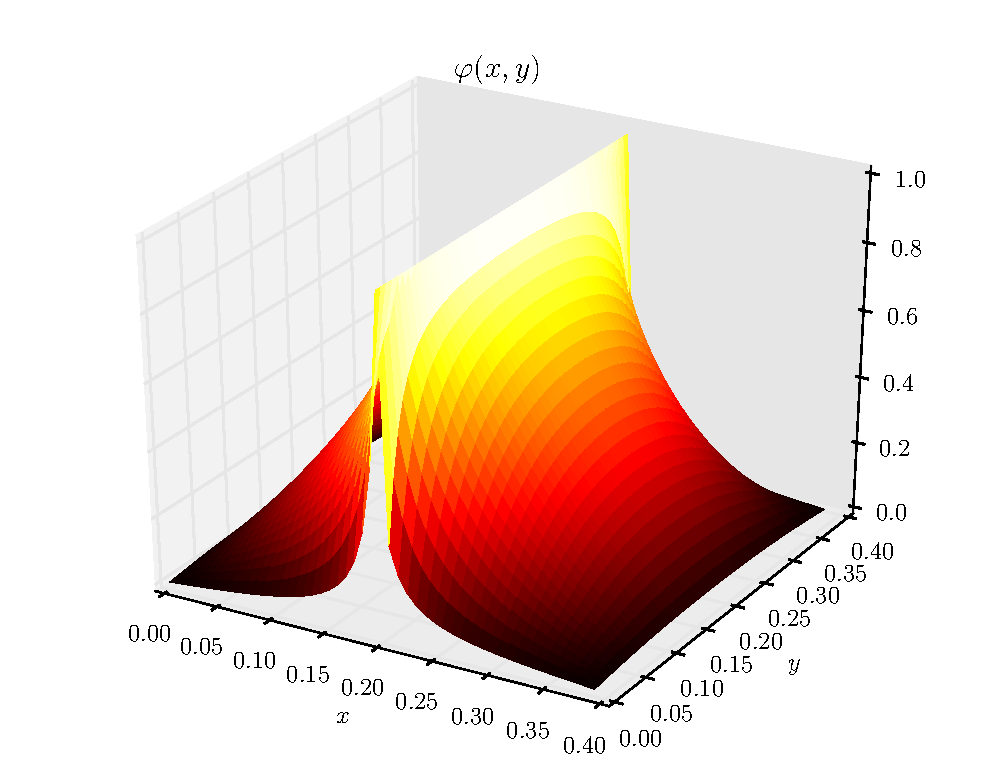
\includegraphics[width=0.3\linewidth]{graphs/examples/plane_surf.eps}
        \label{subfig:plane_surf}
    }
    \subfloat[Vector \textbf{E} field plot]{
        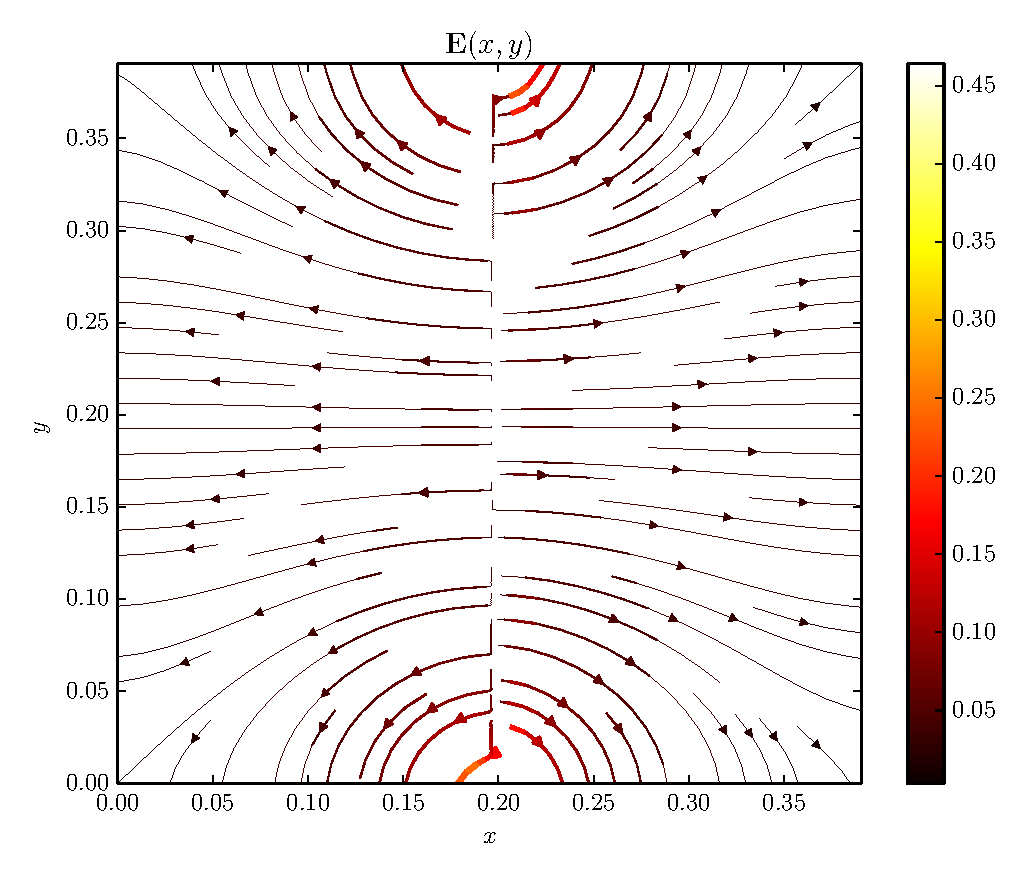
\includegraphics[width=0.3\linewidth]{graphs/examples/plane_vector.eps}
        \label{subfig:plane_vect}
    }
    \caption{Plots of the solution to the Laplace equation with boundary conditions of an equipotential plane.}
    \label{fig:plane}
\end{figure}

\begin{figure}
    \centering
    \subfloat[Contour plot]{
        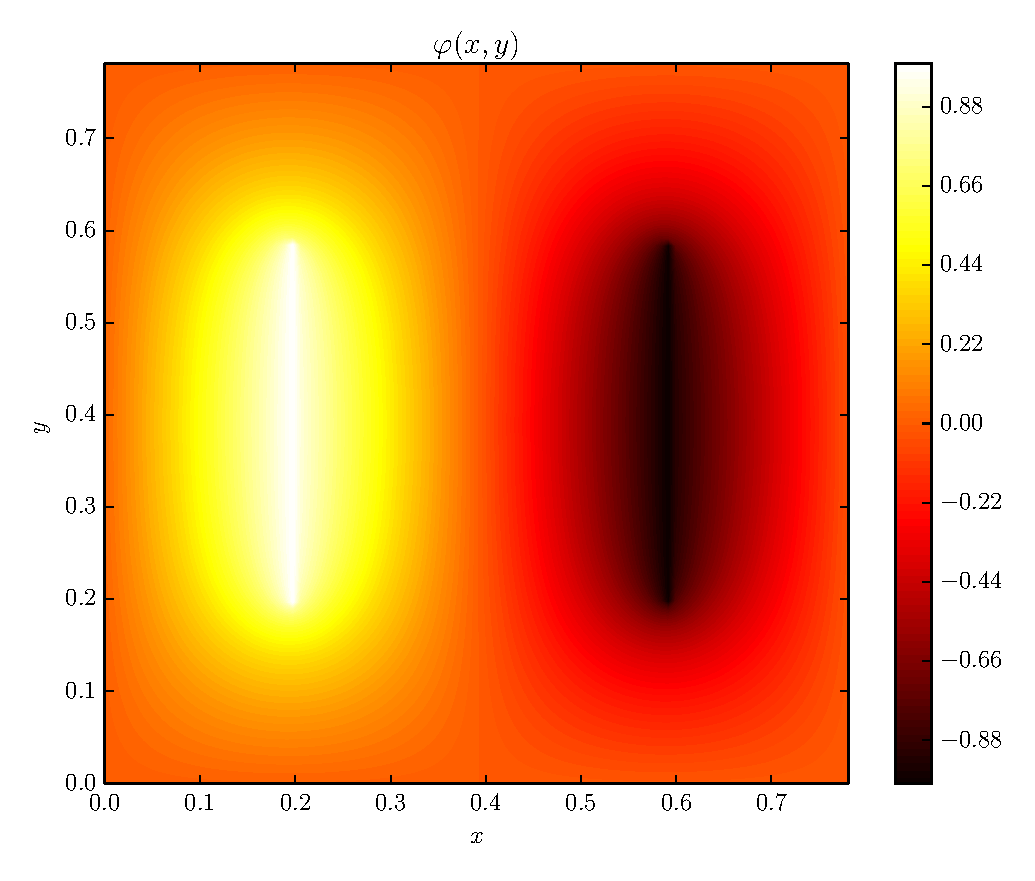
\includegraphics[width=0.3\linewidth]{graphs/examples/capacitor_contour.eps}
        \label{subfig:capacitor_cont}
    }
    \subfloat[Surface plot]{
        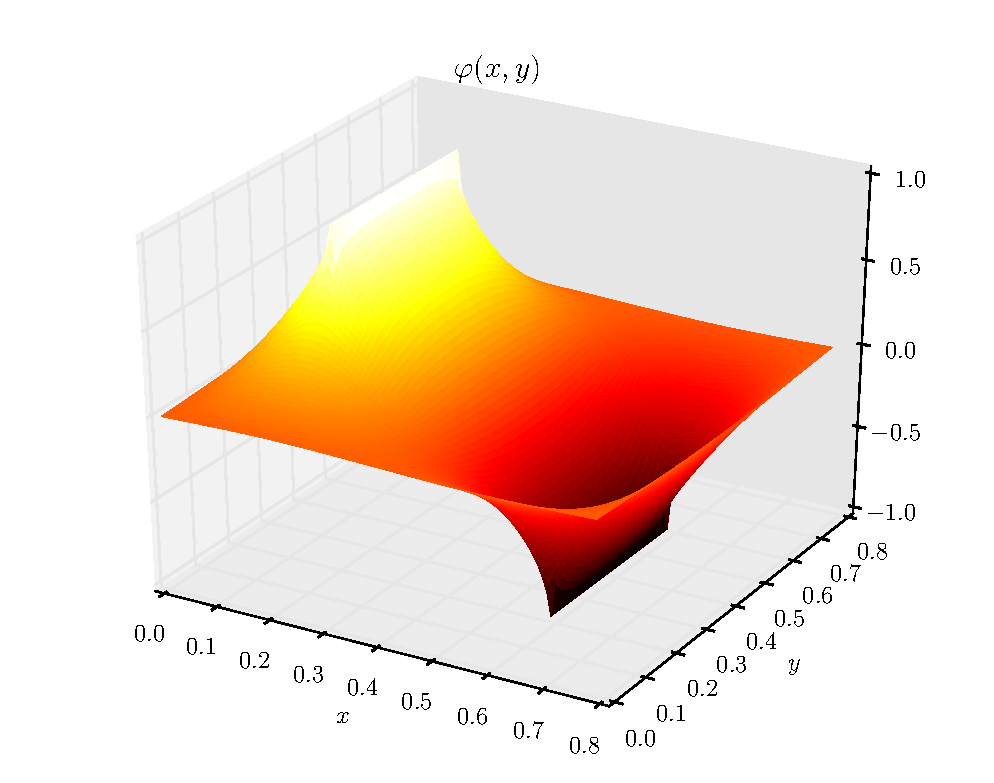
\includegraphics[width=0.3\linewidth]{graphs/examples/capacitor_surf.eps}
        \label{subfig:capacitor_surf}
    }
    \subfloat[Vector \textbf{E} field plot]{
        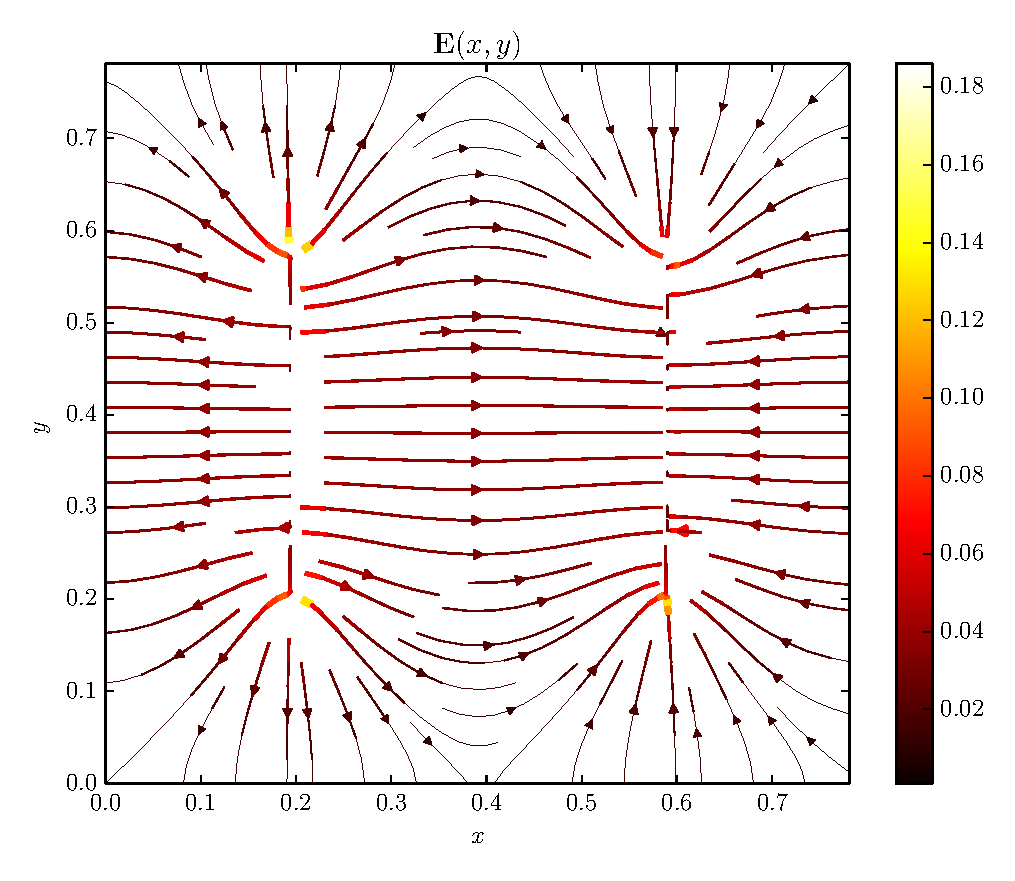
\includegraphics[width=0.3\linewidth]{graphs/examples/capacitor_vector.eps}
        \label{subfig:capacitor_vect}
    }
    \caption{Plots of the solution to the Laplace equation for a parallel plate capacitor.}
    \label{fig:capacitor}
\end{figure}

\begin{figure}
    \centering
    \subfloat[Contour plot]{
        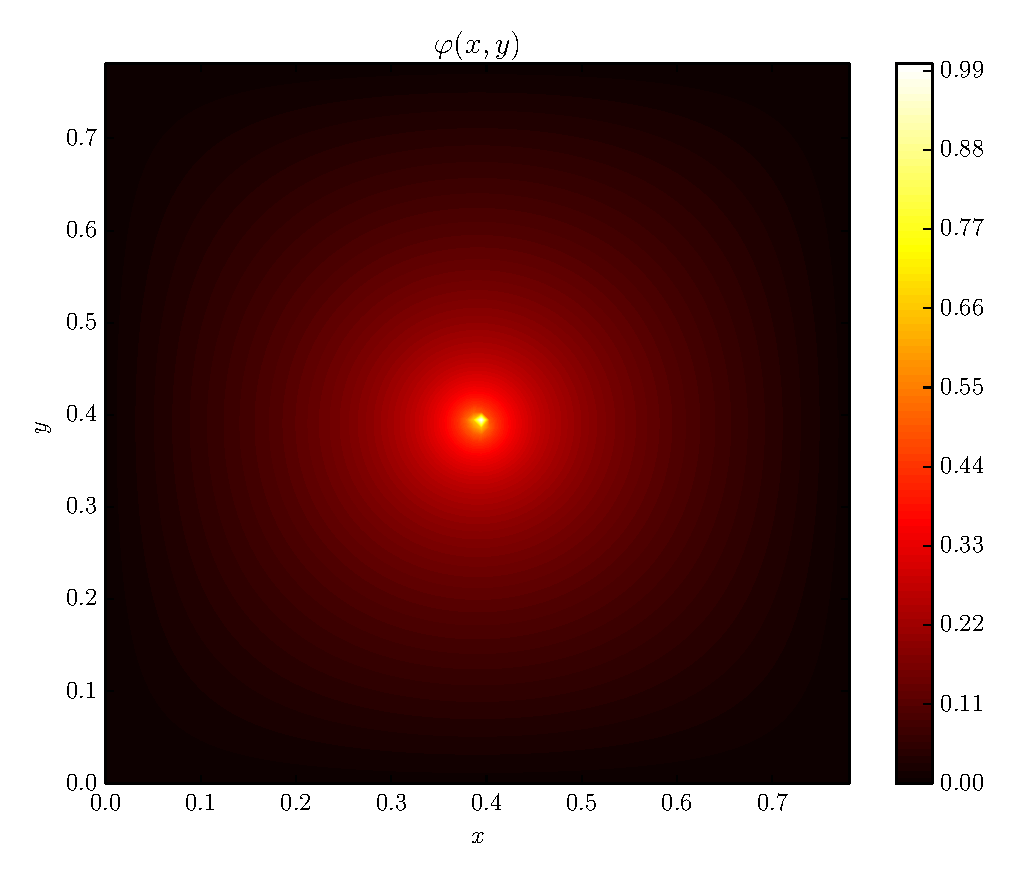
\includegraphics[width=0.3\linewidth]{graphs/examples/point_charge_contour.eps}
        \label{subfig:point_cont}
    }
    \subfloat[Surface plot]{
        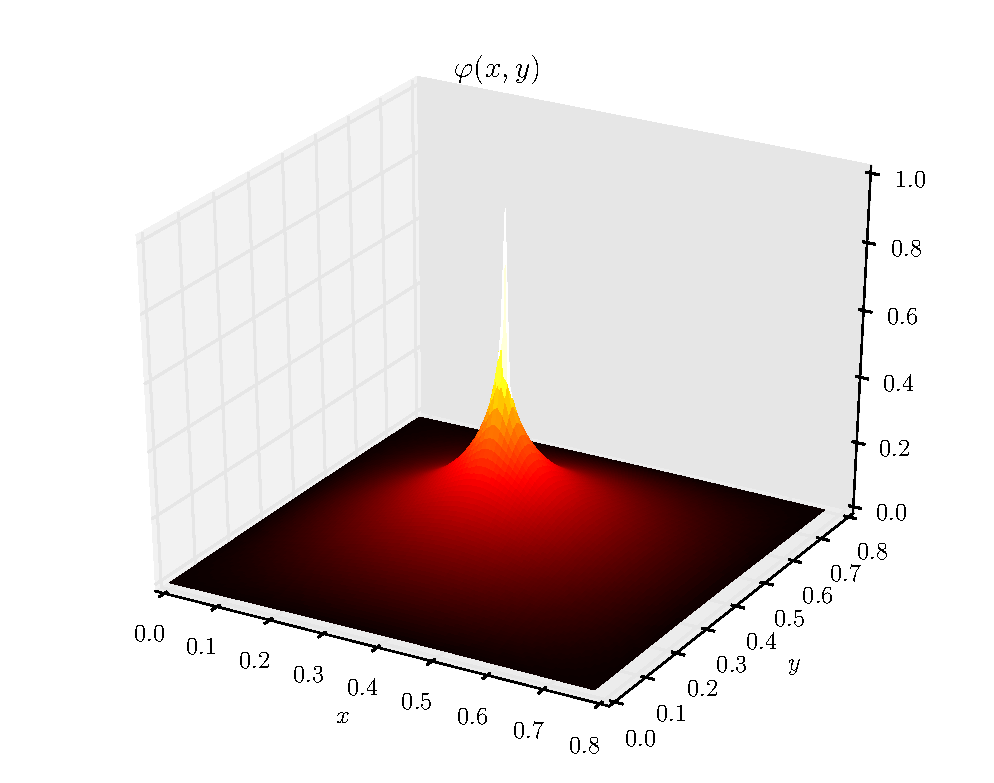
\includegraphics[width=0.3\linewidth]{graphs/examples/point_charge_surf.eps}
        \label{subfig:point_surf}
    }
    \subfloat[Vector \textbf{E} field plot]{
        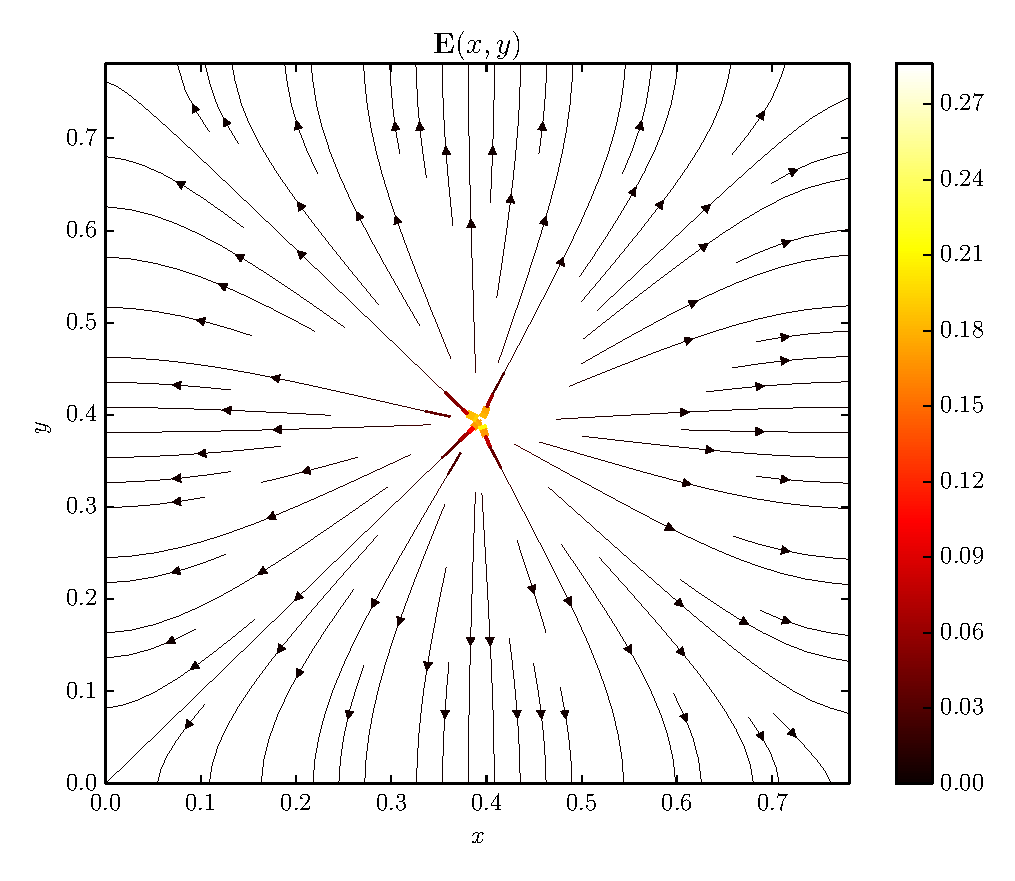
\includegraphics[width=0.3\linewidth]{graphs/examples/point_charge_vector.eps}
        \label{subfig:point_vect}
    }
    \caption{Plots of the solution to the Laplace equation for a single constant potential point.}
    \label{fig:point}
\end{figure}

\begin{figure}
    \centering
    \subfloat[Contour plot]{
        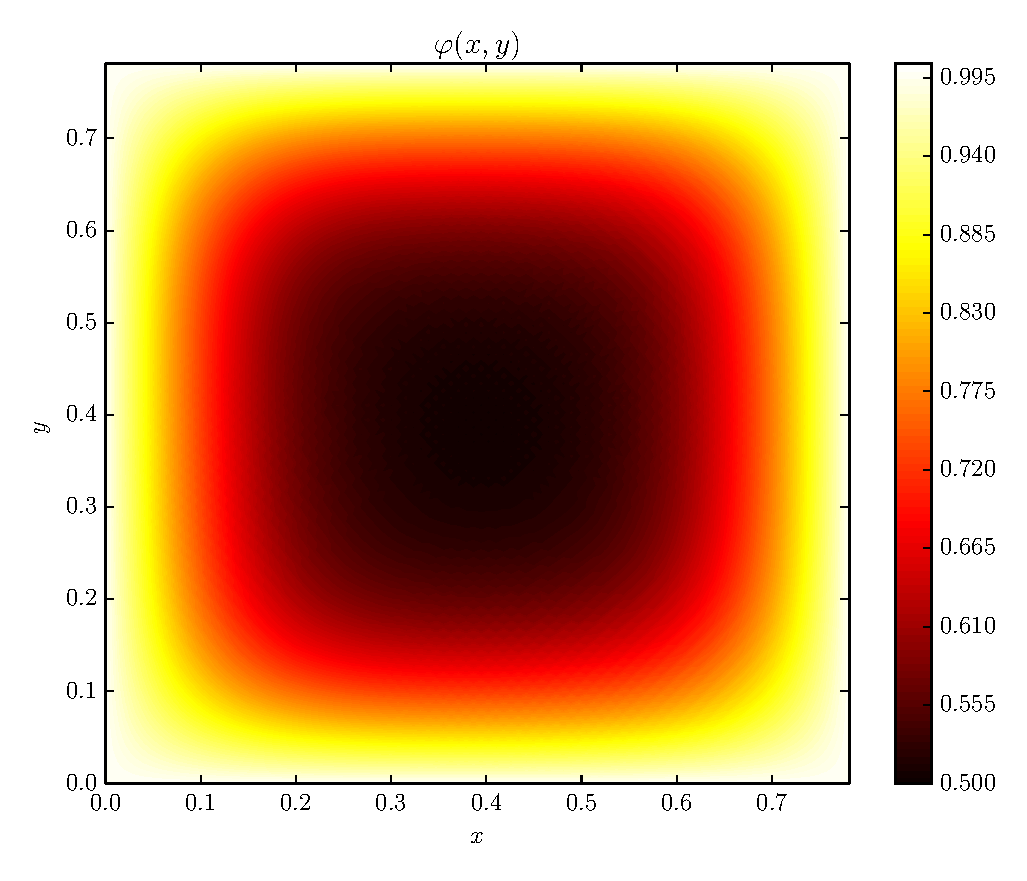
\includegraphics[width=0.3\linewidth]{graphs/examples/net_contour.eps}
        \label{subfig:net_cont}
    }
    \subfloat[Surface plot]{
        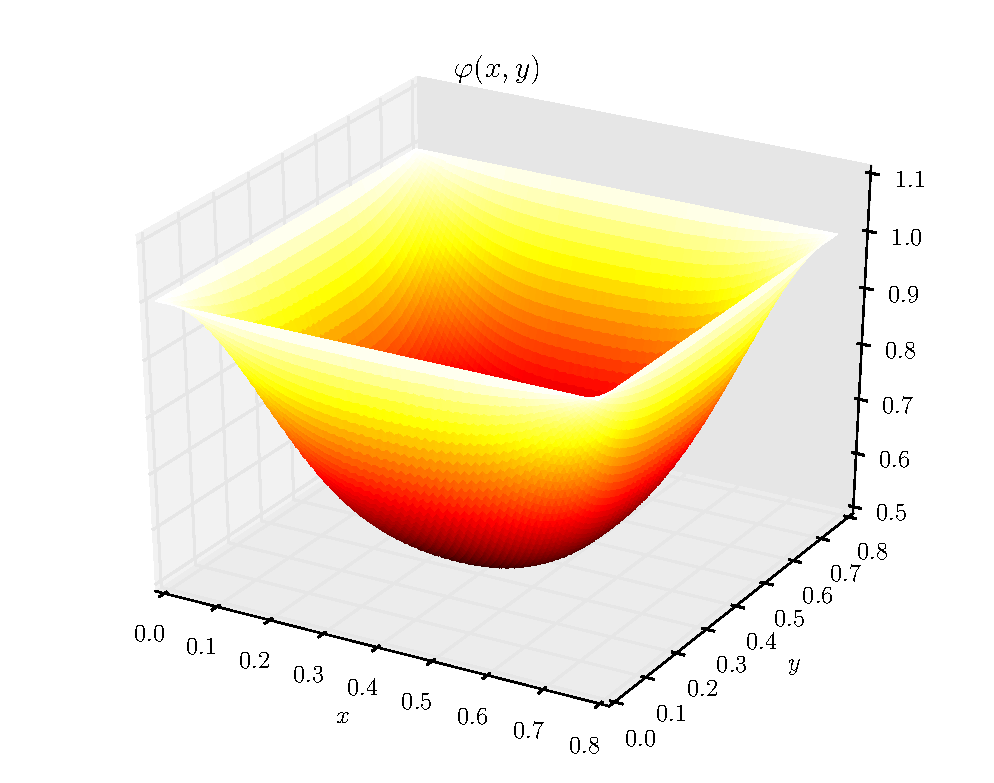
\includegraphics[width=0.3\linewidth]{graphs/examples/net_surf.eps}
        \label{subfig:net_surf}
    }
    \subfloat[Vector \textbf{E} field plot]{
        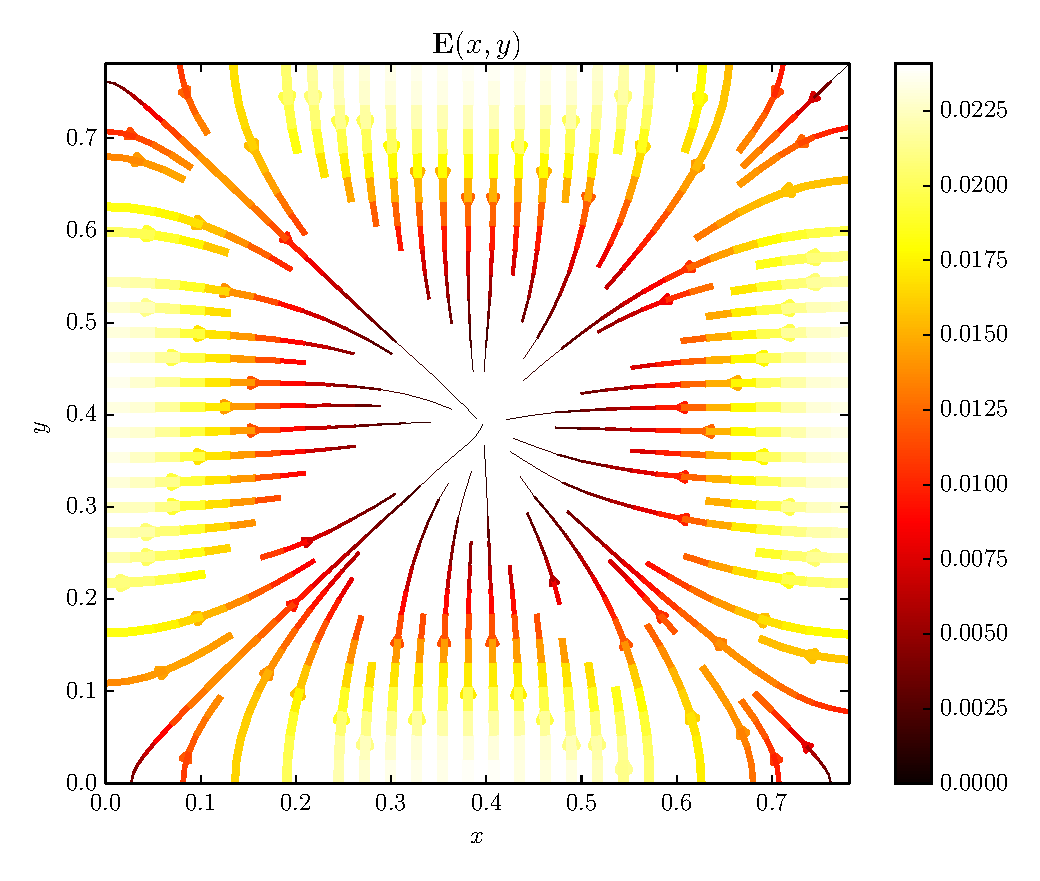
\includegraphics[width=0.3\linewidth]{graphs/examples/net_vector.eps}
        \label{subfig:net_vect}
    }
    \caption{Solution to the Laplace equation with edges of the grid held at constant positive potential.}
    \label{fig:net}
\end{figure}

\begin{figure}
    \centering
    \subfloat[Contour plot]{
        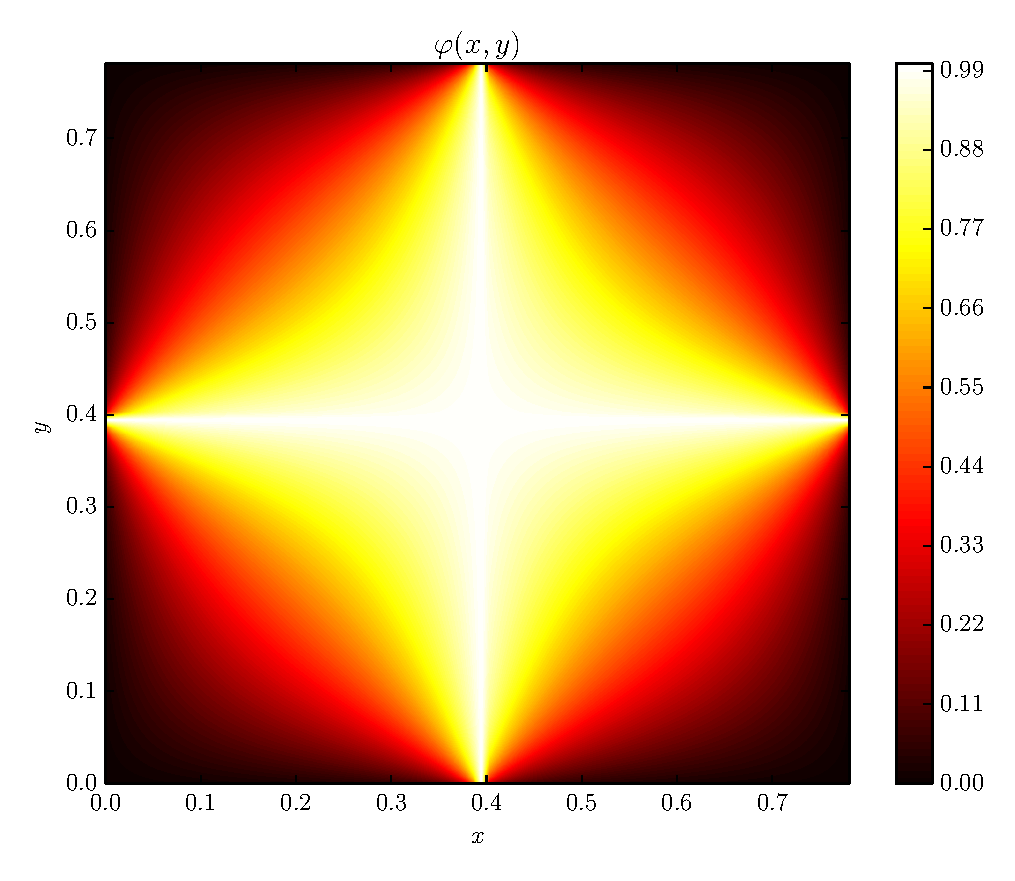
\includegraphics[width=0.3\linewidth]{graphs/examples/cross_contour.eps}
        \label{subfig:cross_cont}
    }
    \subfloat[Surface plot]{
        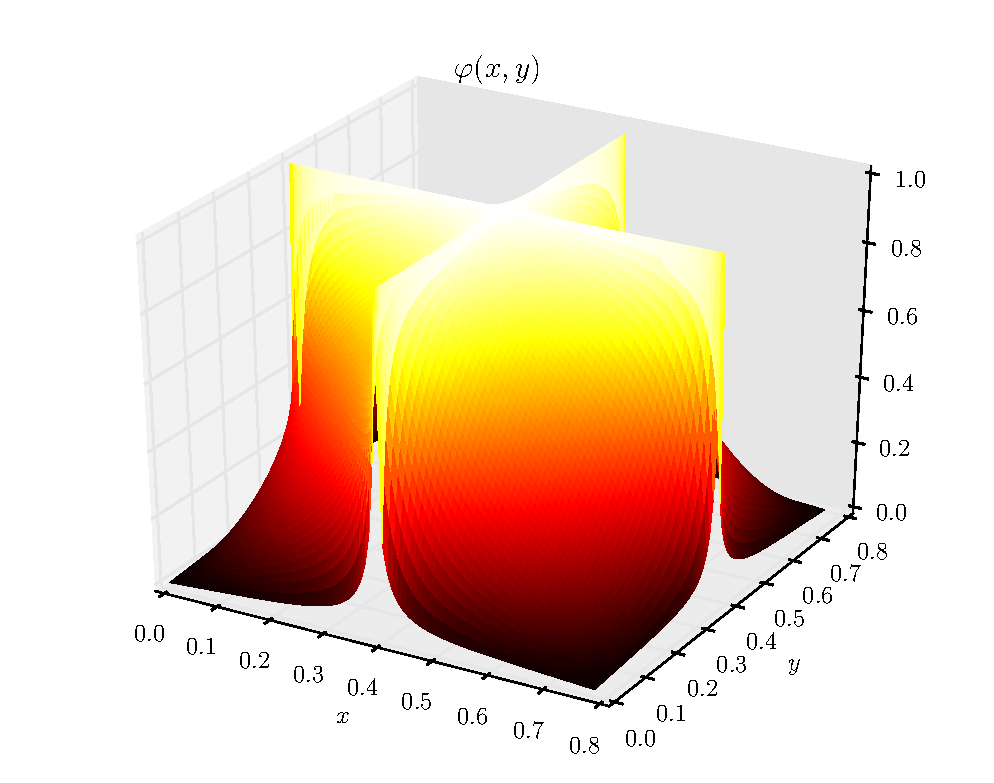
\includegraphics[width=0.3\linewidth]{graphs/examples/cross_surf.eps}
        \label{subfig:cross_surf}
    }
    \subfloat[Vector \textbf{E} field plot]{
        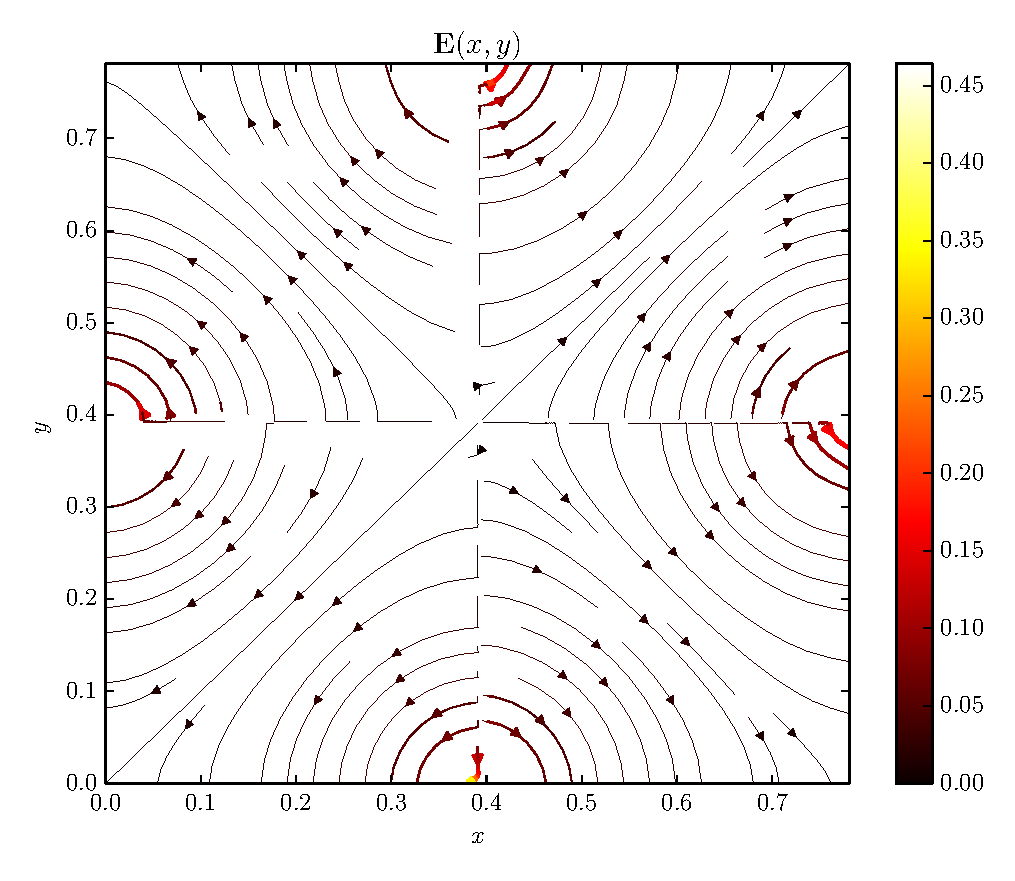
\includegraphics[width=0.3\linewidth]{graphs/examples/cross_vector.eps}
        \label{subfig:cross_vect}
    }
    \caption{Solution to the Laplace equation with equipotential cross overlaid on grid.}
    \label{fig:cross}
\end{figure}

\subsection{Convergence Condition}
\label{subsec:convergence_condition}

An absolute convergence condition is implemented to decide when the program has successfully iterated to the solution of the Laplace equation with the set boundary conditions. As compared to a relative convergence conditions, e.g. that no value changes by more than $X\%$, this has the disadvantage of depending on the boundary conditions applied to the system. So an absolute error tolerance of $\epsilon = \SI{0.01}{V}$ may be appropriate if the highest boundary condition is $\mathcal{O}(\SI{100}{V})$, but inappropriate if the potential boundary condition is $\mathcal{O}(\SI{0.1}{V})$. This is compensated for by the ability to manually change the error tolerance with the \texttt{--error} flag. By default this value is set at $10^{-4}$. When the boundary conditions are a single constant potential of \SI{1}{V} at the centre of the grid, the effect of a relatively large tolerance is to fatten the potential field around the point in the centre, as shown in Figure \ref{fig:tolerances}. This is because a too high $\epsilon$ means the iterations stop before a true solution is found. As there are no charges involved, the effect of each iteration is merely to average from the surrounding nodes. Hence when the program finishes the iterations early, it means it has prematurely ceased this averaging process and thus is higher near the central peak than it should physically be.

Increasing the absolute tolerance does, however, radically decrease the time taken and number of iterations needed to converge. Figure \ref{subfig:error_1e-2}, with $\epsilon = 10^{-2}$ on a grid of 100 by 100 took 95.56 seconds and 1815 iterations to converge, whilst Figure \ref{subfig:error_1e-6} took 784.33 seconds and 13789 iterations to converge. There is thus a trade off between time taken to converge and the precision of the convergent solution, as would be expected. Note that the average time taken per iteration, at 52.7 and 56.8 milliseconds for $\epsilon = 10^{-2}$ and $\epsilon = 10^{-6}$ respectively, is roughly unchanged.

\begin{figure}
    \centering
    \subfloat[$\epsilon = 10^{-2}$]{
        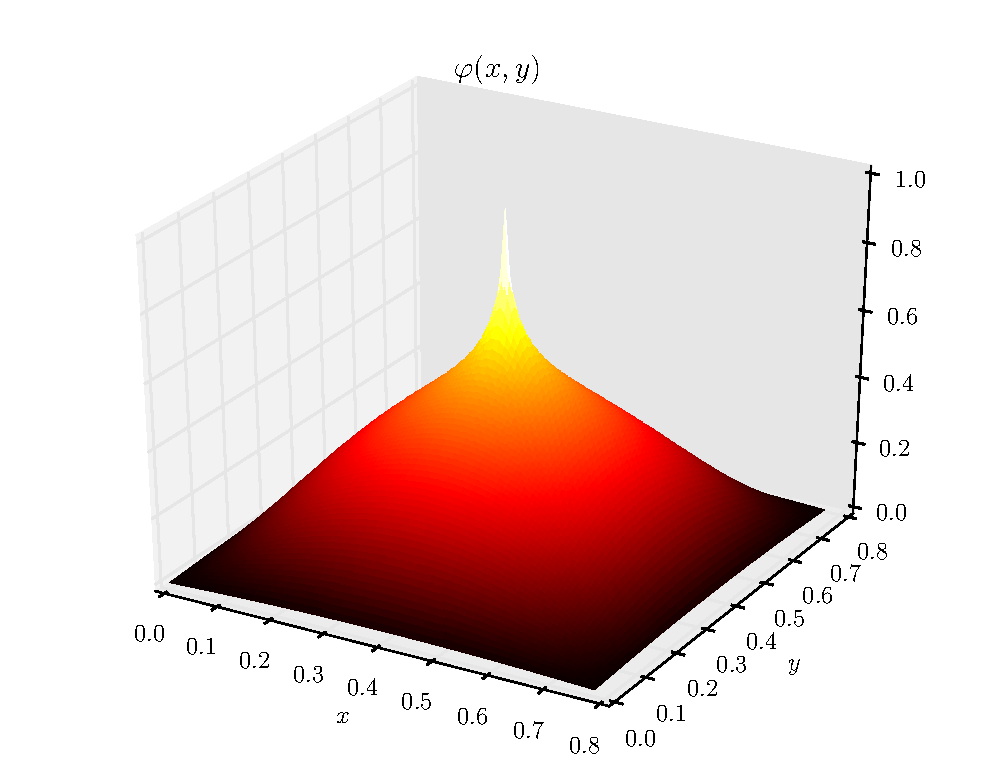
\includegraphics[width=0.5\linewidth]{graphs/tolerance/point_charge_error_1e-2_surf.eps}
        \label{subfig:error_1e-2}
    }
    \subfloat[$\epsilon = 10^{-6}$]{
        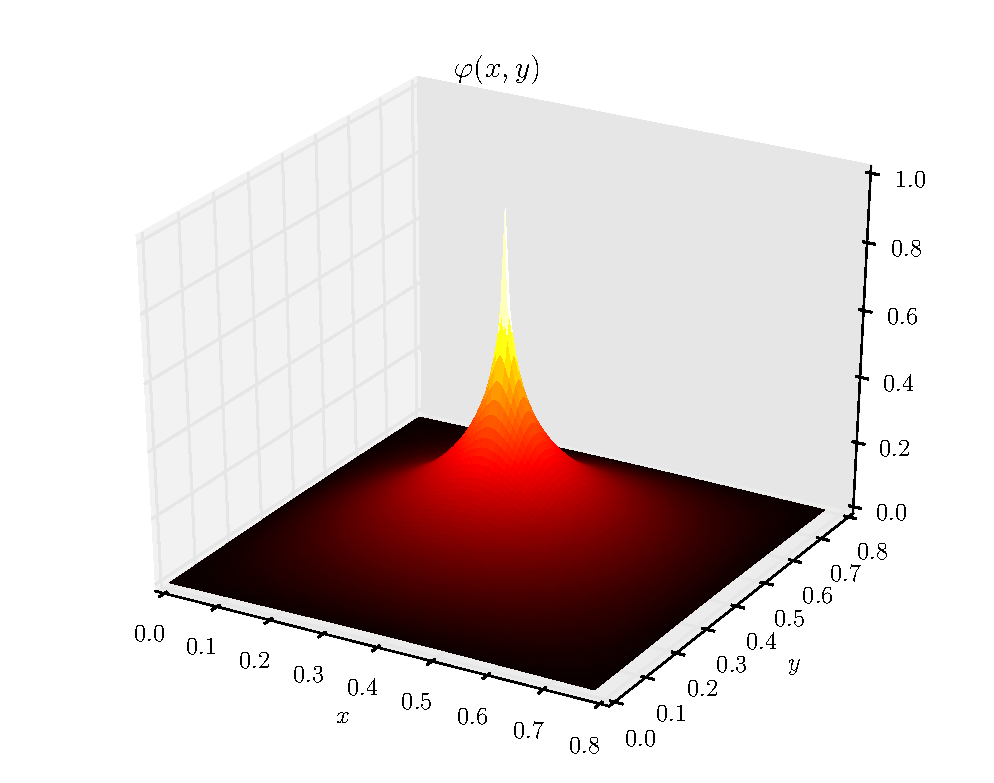
\includegraphics[width=0.5\linewidth]{graphs/tolerance/point_charge_error_1e-6_surf.eps}
        \label{subfig:error_1e-6}
    }
    \caption{Comparison of the effect of altering the absolute error tolerance, $\epsilon$, in the convergence condition on the resulting solution.}
    \label{fig:tolerances}
\end{figure}

\subsection{Iteration Method}
\label{subsec:iteration_method}

Both the Jacobi and Gauss-Seidel iteration methods are implemented, with the option of which to use left up to the user with the positional argument \texttt{method} determining which to use. Surprisingly, the Gauss-Seidel and Jacobi show no statistically significant changes in the time taken to converge or number of iterations needed to converge. When tested 20 times on a 100 by 100 grid, using the boundary conditions of the parallel plate capacitor as a test case, the Jacobi method averaged $313.78 \pm 63.39$ seconds of processor time and $4045 \pm 601$ iterations as compared to the Gauss-Seidel method, which took $319.23 \pm 55.27$ seconds and $4120 \pm 664$ iterations. Equally, when tested using different boundary conditions and grid densities, there consistently is no significant performance difference between the two. For a plane equipotential on a 32 by 32 grid averaging from 20 runs, Jacobi takes $2.94 \pm 0.28$ processor seconds and $537 \pm 48$ iterations, whilst Gauss-Seidel requires $3.00 \pm 0.34$ seconds and $555 \pm 61$ iterations, well within each others' standard error. This is contrary to popular presentations of the Gauss-Seidel method as the slightly faster of the two \cite{edwards2004,golub1996}, although no such general result can be said to hold \cite{demmel1997}. The two methods produce identical convergent results given the same input variables, as would be expected.
\subsection{Grid Density}
\label{subsec:grid_density}

The default parameters of the grid density are a 50 by 50 grid. Changing the density significantly increases the time taken to find a converging solution. In particular combining high density with very low tolerance results in extremely long convergence times, as shown by the fact that Figure \ref{subfig:error_1e-6} with a grid density of 100 by 100 and absolute error tolerance of $\epsilon = 10^{-6}$ took 784.33 processor seconds and 13789 iterations to converge, whilst with the much lower grid density of 32 by 32, again with $\epsilon = 10^{-6}$, convergence takes only 9.48 processor seconds and 1651 iterations, significantly lower. This also demonstrates that an increase in grid density significantly increases the processor time taken to run each iteration. For 100 by 100 grid with $\epsilon = 10^{-6}$, each iteration on average took 56.9 milliseconds, whilst for the 32 by 32 grid with $\epsilon = 10^{-6}$, each iteration took only 5.7 milliseconds. This means this increase in grid density resulted in an increase in the time taken to complete each iteration by a factor of ten. This implies that while the convergence condition affects the number of iterations needed to converge, it does not affect the time taken per iteration, whilst the grid density increases the time taken per iteration. This makes sense because the convergence condition only makes more stringent the requirement that classifies when the solution has been found and iterations can stop, whilst the grid density increases the number of nodes that need to be evaluated by finite difference for each iteration (which spans the whole grid).

\subsection{Grid Edges}
\label{subsec:grid_edges}

The problem arises when using the iteration formula given in Equation \ref{eqn:iteration} that when iterating at the edges of the grid, i.e. when grid indices $i=0$ or $j=0$, there are not four neighbouring nodes to include in the iteration. The approximation is made that these nodes outside of the grid can be taken as zero, as opposed to averaging over the neighbouring nodes that are within the grid. This is an acceptable approximation because it produces similar if not identical results and converges significantly faster. Figure \ref{fig:grid_edges} shows a comparison of the potential field around a constant potential point whilst making the assumption and without making the assumption (i.e. averaging over the nodes within the grid only). As can be seen, the two results are nearly identical, with the minor difference that Figure \ref{subfig:no_assume} has serrated grid edges. This is an artefact of the edges not having the full four neighbouring nodes to average from. However, the solution in Figure \ref{subfig:no_assume} took 218.92 seconds of processor time and 3908 iterations to converge, taken from an average of 10 runs, whilst \ref{subfig:assume} took only 26.42 processor seconds and 519 iterations, again from an average of 10 runs. These tests were done using the Gauss-Seidel iteration method. Given that this is a factor of 8 times faster, requiring 7.5 times fewer iterations to converge, to produce very similar results, the assumption is justifiable.

\begin{figure}
    \centering
    \subfloat[Making the assumption]{
        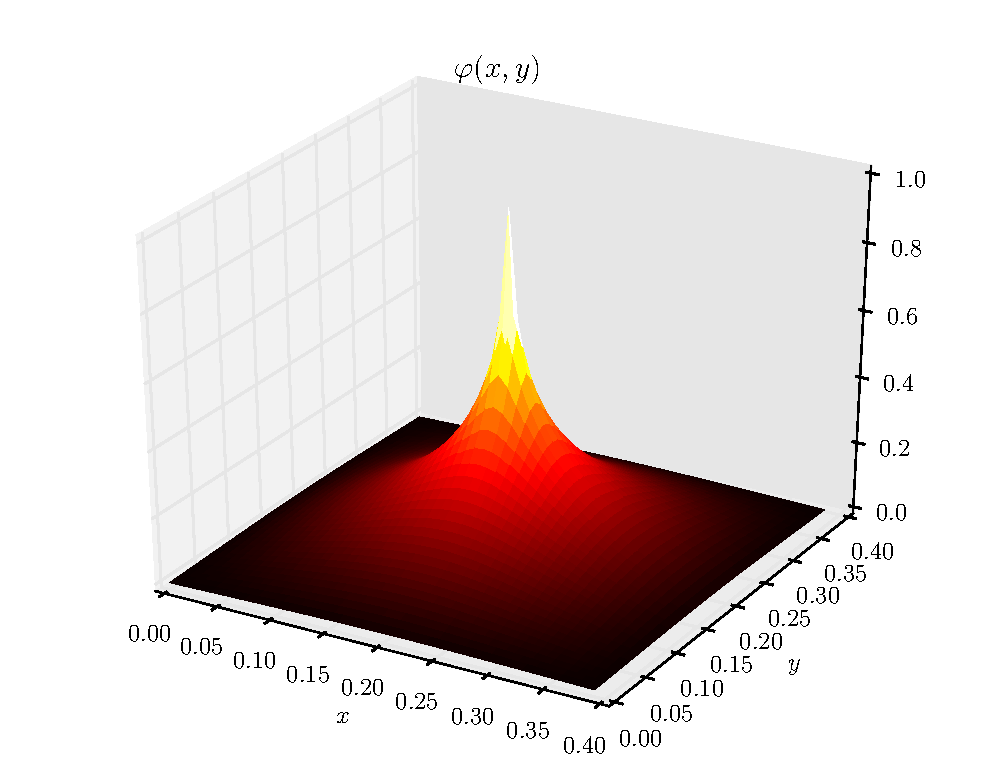
\includegraphics[width=0.5\linewidth]{graphs/grid_edges/assume_50x50_error_1e-4_surf.eps}
        \label{subfig:assume}
    }
    \subfloat[Without making the assumption]{
        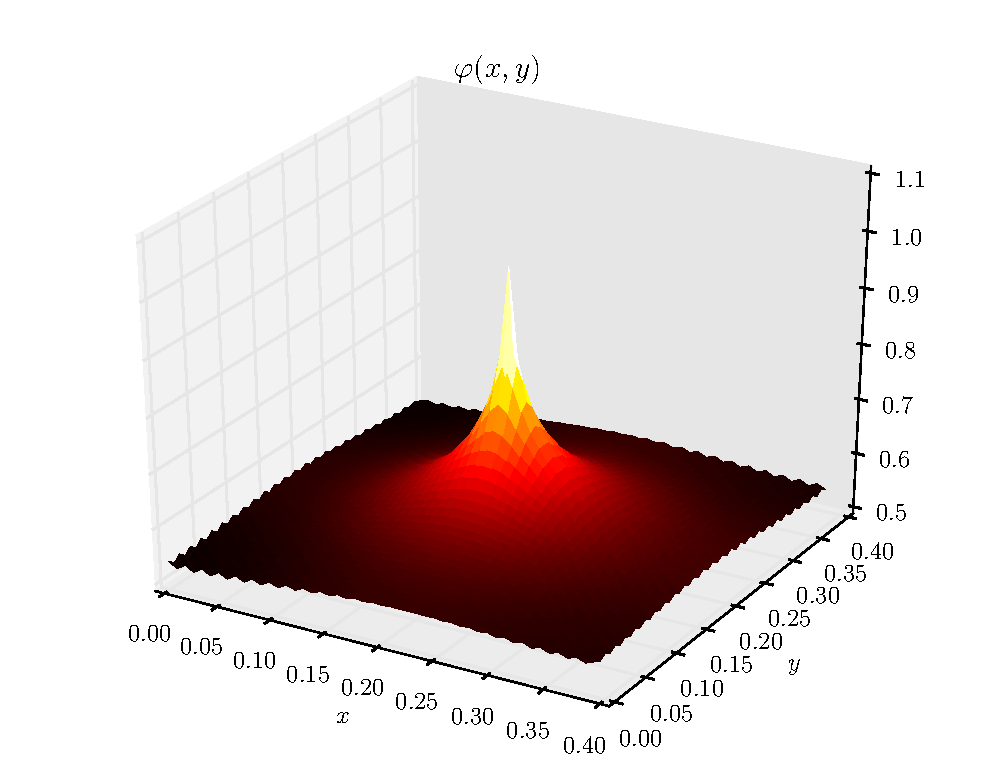
\includegraphics[width=0.5\linewidth]{graphs/grid_edges/no_assume_50x50_error_1e-2_surf.eps}
        \label{subfig:no_assume}
    }
    \caption{A comparison of the results produced by the Gauss-Seidel method when making the assumption that non-grid nodes are zero and without making the assumption.}
    \label{fig:grid_edges}
\end{figure}

\section{Calculating Potential and Electric Field of Parallel Plate Capacitor}
\label{sec:parallel_plate_capacitor}

Next the program to solve Laplace's equation in two dimensions is applied to two equipotential plates, i.e. a parallel plate capacitor. The potential and electric fields are plotted in Figures \ref{subfig:capacitor_surf_big} and \ref{subfig:capacitor_vector_big}. Figure \ref{subfig:capacitor_surf_big} shows that between the positive plate on the left and the negative plate on the right, the surface of the potential field has a constant gradient. Figure \ref{subfig:capacitor_vector_big} also demonstrates clearly that between the two plates, the electric field is linear and constant, as is expected. Around the ends of the plates it can also be seen that the infinite plate approximation breaks down and the field lines curve away from the region of constant electric field strength.

\begin{figure}
    \centering
    \subfloat[Surface plot.]{
        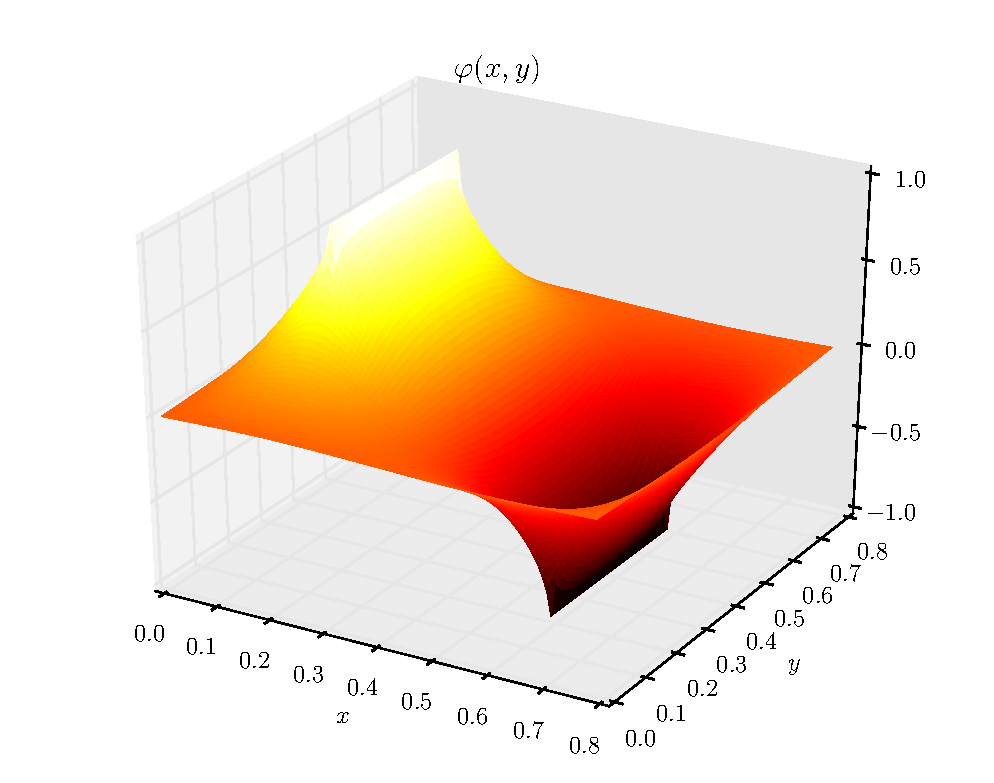
\includegraphics[width=0.5\linewidth]{graphs/examples/capacitor_surf}
        \label{subfig:capacitor_surf_big}
    }
    \subfloat[Electric field lines plot.]{
        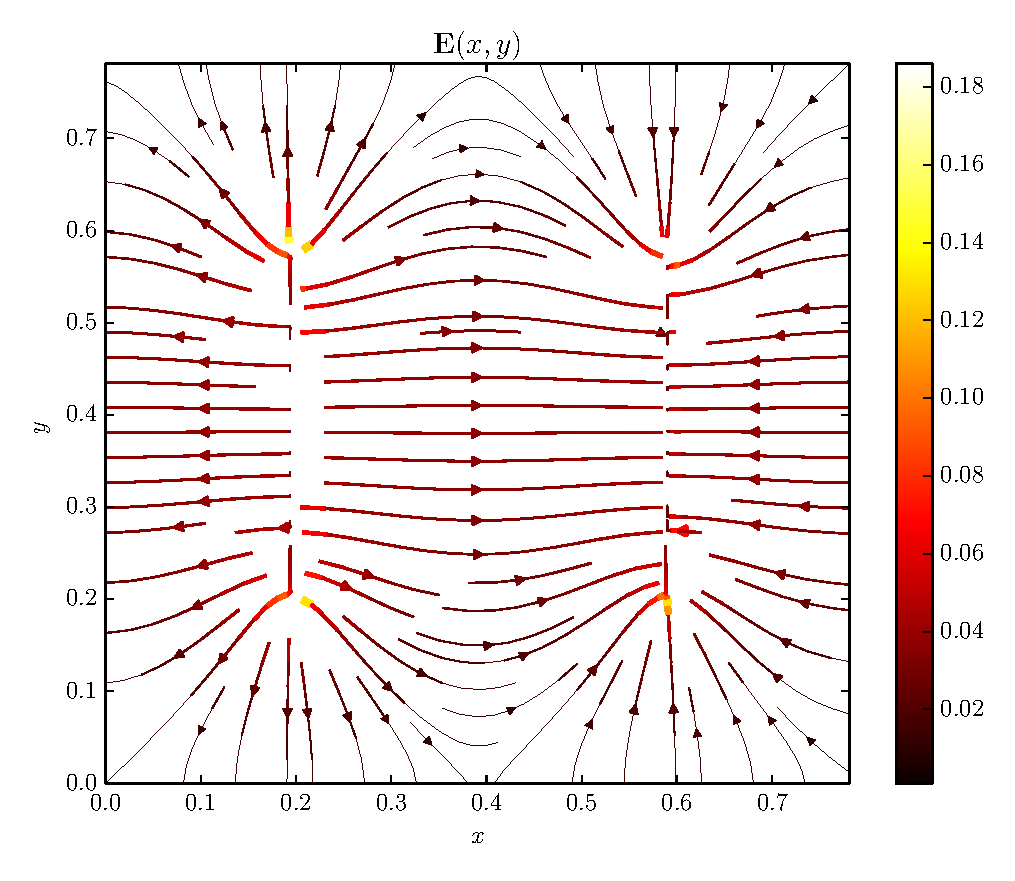
\includegraphics[width=0.5\linewidth]{graphs/examples/capacitor_vector}
        \label{subfig:capacitor_vector_big}
    }
    \caption{Surface plot of the solution to Laplace's equation in and around a parallel plate capacitor.}
    \label{fig:capacitor_big}
\end{figure}

\subsection{Infinite Plate Solution}
\label{subsec:infinite_plate_solution}

When the distance between the plates, $d$, is large compared to the width of the capacitor plates, $a$, the capacitor looks like a dipole, as shown in Figures \ref{subfig:small_capacitor_contour} and \ref{subfig:small_capacitor_magnitude}. As the plates are brought closer together and the width increases, i.e. the ratio $\frac{a}{d}$ increases, the solution looks more and more like the infinite plate solution, namely $E=0$ outside the capacitor and $E = \frac{V}{d}$ inside the capacitor. Figures \ref{subfig:long_capacitor_contour} and \ref{subfig:long_capacitor_magnitude} shows a wide parallel plate capacitor where the plates are very close together. As can clearly be seen, both the potential surface and the electric field lines corroborate the infinite plate solution inside the capacitor, where the potential surface is an inclined plane and the electric field lines are straight lines from positive plate to negative plate. Figure \ref{subfig:long_capacitor_magnitude} shows that when $\frac{a}{d}$ is large, the magnitude of the field outside the capacitor goes almost completely to zero. Quantitatively, if a potential difference of \SI{2}{V} is maintained between two capacitor plates 4 nodes apart ($d=4$ nodes) with width 98 nodes ($a=98$ nodes) with grid density 100 by 100, as shown in Figures \ref{subfig:long_capacitor_contour} and \ref{subfig:long_capacitor_magnitude}, then the average electric field strength outside the plates is \SI{0.02}{\volt} and inside the plates is \SI{0.49}{\volt}. As $E=\frac{V}{d}=1/2$, this is extremely close to the infinite plate solution. The slight offset from this infinite plate solution is due to the edges of the plates having slightly lower electric field strength than in between the plates, as can be seen in Figure \ref{subfig:long_capacitor_magnitude}. The calculated solution to the Laplace equation for a parallel plate capacitor thus approximates the infinite plate solution extremely well when the ratio of the plate width to separation is large.

\begin{figure}
    \centering
    \subfloat[Small $\frac{a}{d}$.]{
        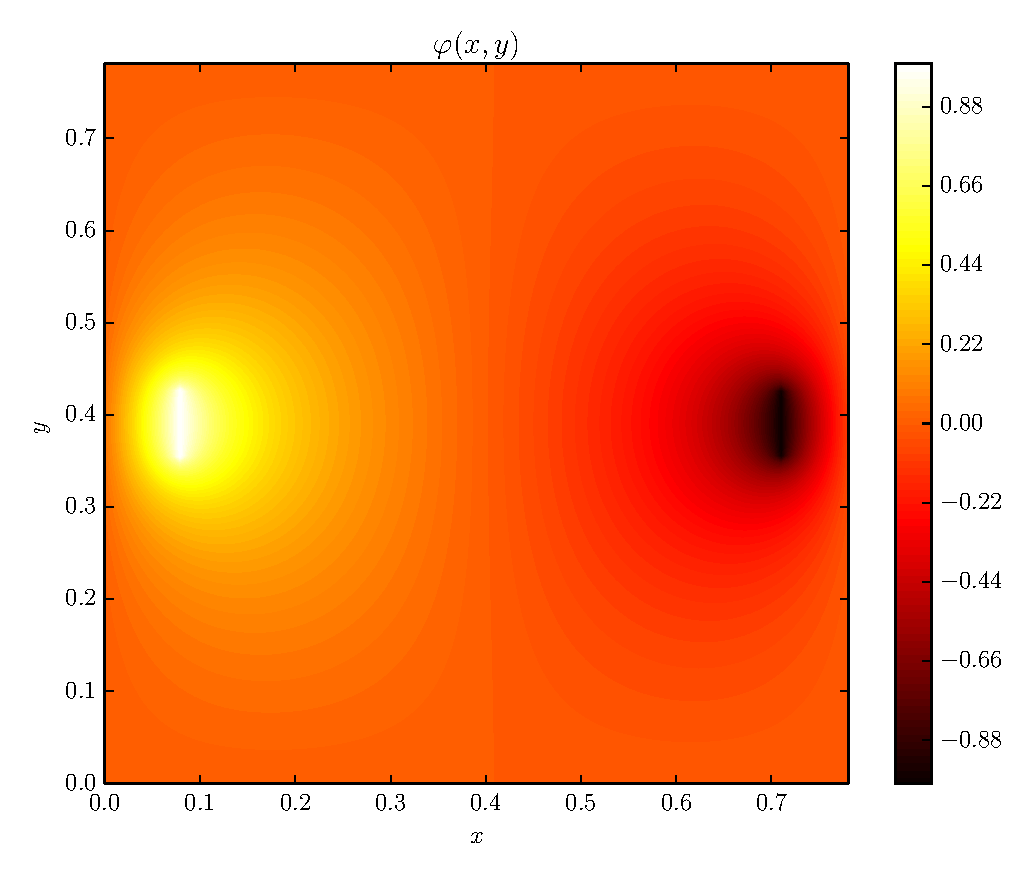
\includegraphics[width=0.5\linewidth]{graphs/capacitor/small_capacitor_contour}
        \label{subfig:small_capacitor_contour}
    }
    \subfloat[Large $\frac{a}{d}$.]{
        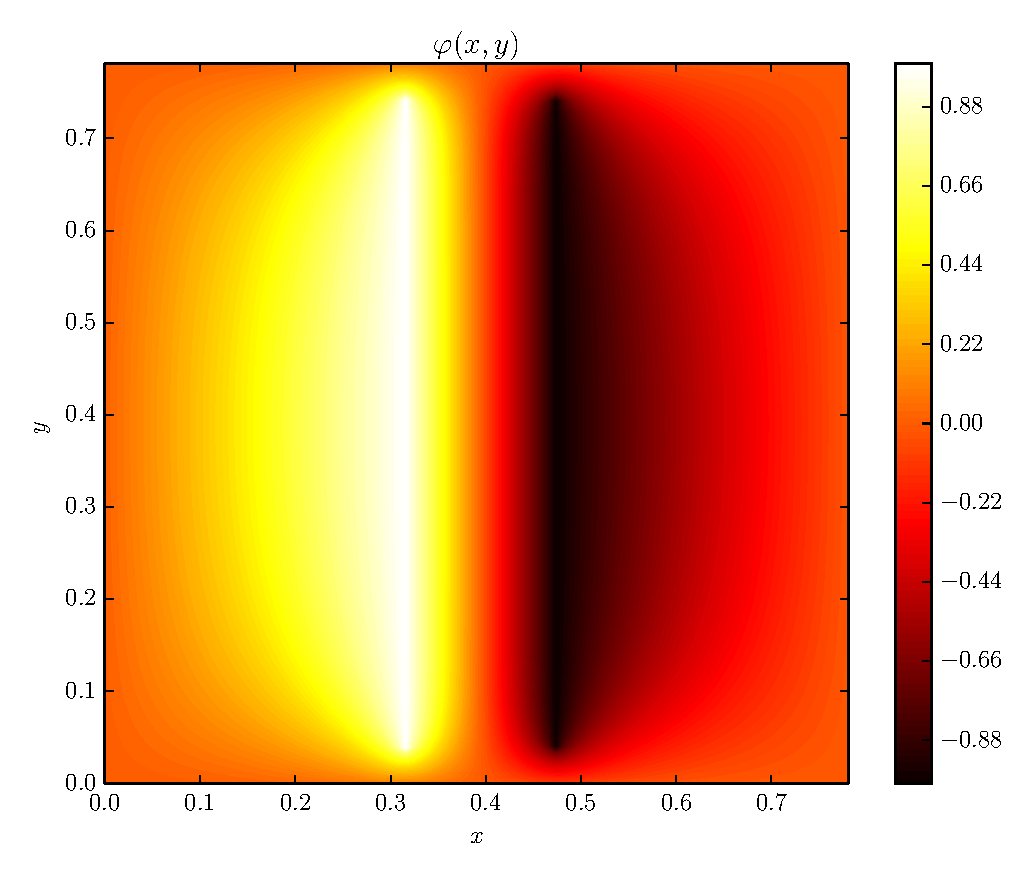
\includegraphics[width=0.5\linewidth]{graphs/capacitor/long_capacitor_contour}
        \label{subfig:long_capacitor_contour}
    }
    \caption{The potential field contours around a parallel plate capacitor for small and large $\frac{a}{d}$.}
    \label{fig:capacitor_sizes_contour}
\end{figure}

\begin{figure}
    \centering
    \subfloat[Small $\frac{a}{d}$.]{
        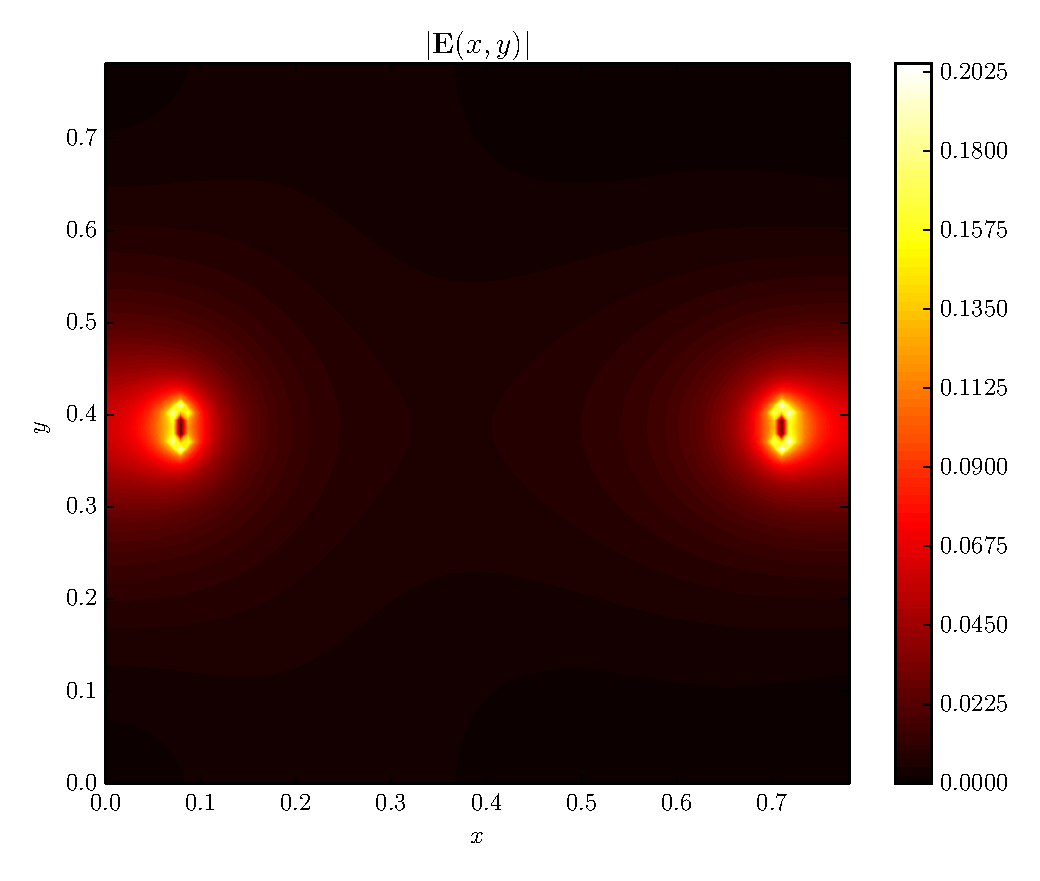
\includegraphics[width=0.5\linewidth]{graphs/capacitor/small_capacitor_magnitude}
        \label{subfig:small_capacitor_magnitude}
    }
    \subfloat[Large $\frac{a}{d}$.]{
        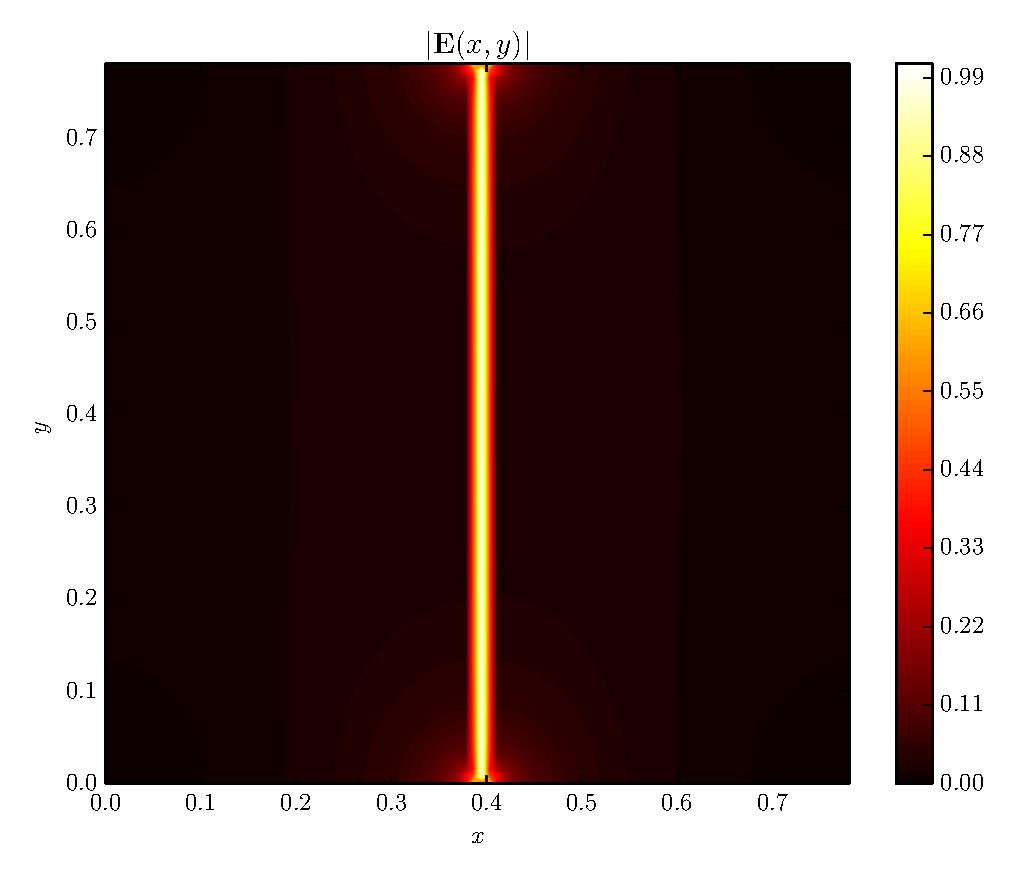
\includegraphics[width=0.5\linewidth]{graphs/capacitor/long_capacitor_magnitude}
        \label{subfig:long_capacitor_magnitude}
    }
    \caption{The magnitude of the electric field contours around a parallel plate capacitor for small and large $\frac{a}{d}$.}
    \label{fig:capacitor_sizes_magnitude}
\end{figure}

\section{Solving the Diffusion Equation for Iron Poker}
\label{sec:diffusion_equation}

In the final section of the exercise, the heat diffusion equation is solved for a metal rod. The heat diffusion equation is given by:
\begin{equation}
    \alpha \nabla^2 \phi = \frac{\partial \phi}{\partial t},
\end{equation}
where $\alpha = \frac{k}{\rho c_p}$ (with $k$ the the thermal conductivity, $\rho$ the density and $c_p$ the specific heat capacity) is the thermal diffusivity and $\phi$ is the temperature. Two boundary conditions are solved for: firstly, one end in a hot furnace of \SI{1000}{\celsius} only, and the other with one end in a hot furnace of \SI{1000}{\celsius} and the other in cold ice at \SI{0}{\celsius}. Heat loss through the edges of the rod are ignored throughout.

\subsection{One end held in furnace at \SI{1000}{\celsius}}
\label{subsec:hot}

Firstly, one end of the rod is held in a furnace of temperature \SI{1000}{\celsius}, and no heat is lost through the end of the poker. The result of letting time advance is thus to let heat gradually dissipate up through the rod to the other end of the rod. Because no heat is lost, heat continues to build up indefinitely until the entire rod is at \SI{1000}{\celsius}. Whilst the rod will never in a finite time reach this equithermal point, the entire rod is at the same temperature to an absolute error tolerance of $\epsilon = 10^{-4}$\si{\kelvin} after 261,322 iterations with step size \SI{0.1}{\second}, i.e. after \SI{26,132}{\second}. Figures \ref{fig:hot_diffusion} show the one-dimensional temperature distribution along the rod as time advances.

\begin{figure}
    \centering
    \subfloat[$t=$\SI{10}{\second}]{
        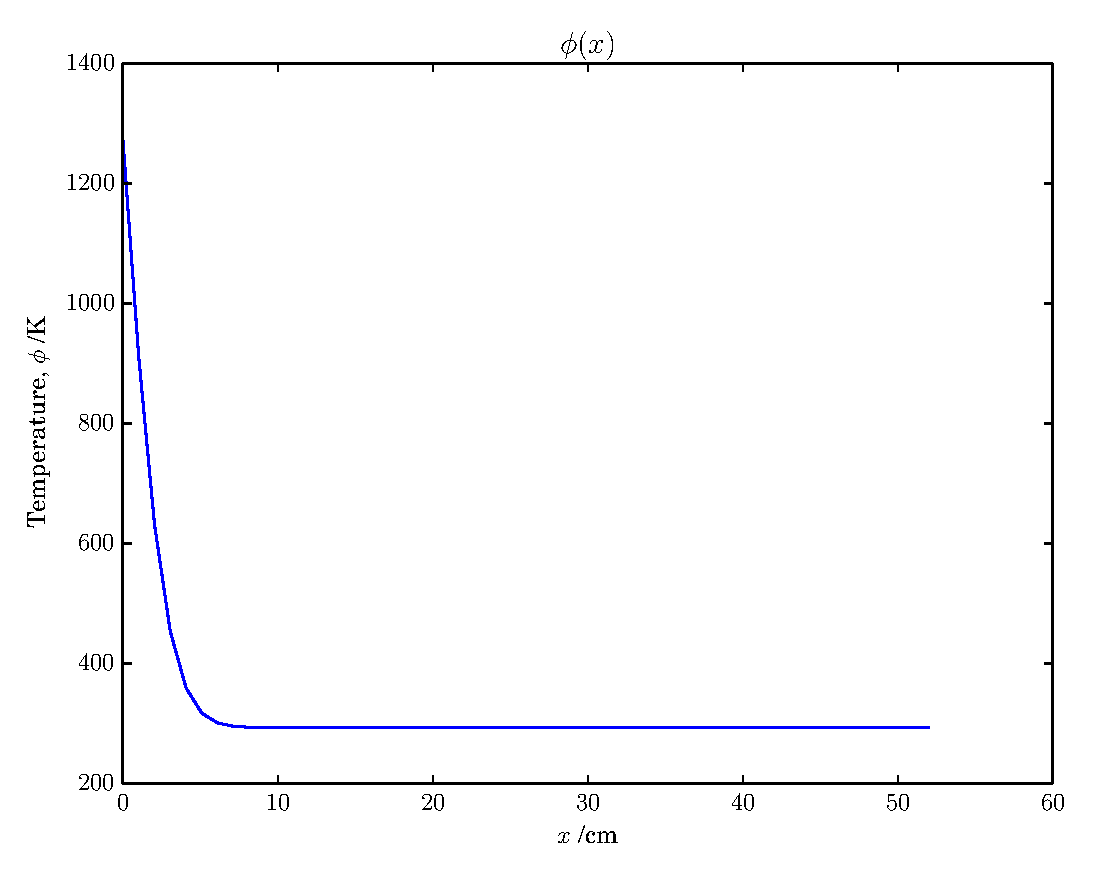
\includegraphics[width=0.5\linewidth]{graphs/diffusion/hot/t_10_rod_normal}
    }
    \subfloat[$t=$\SI{100}{\second}]{
        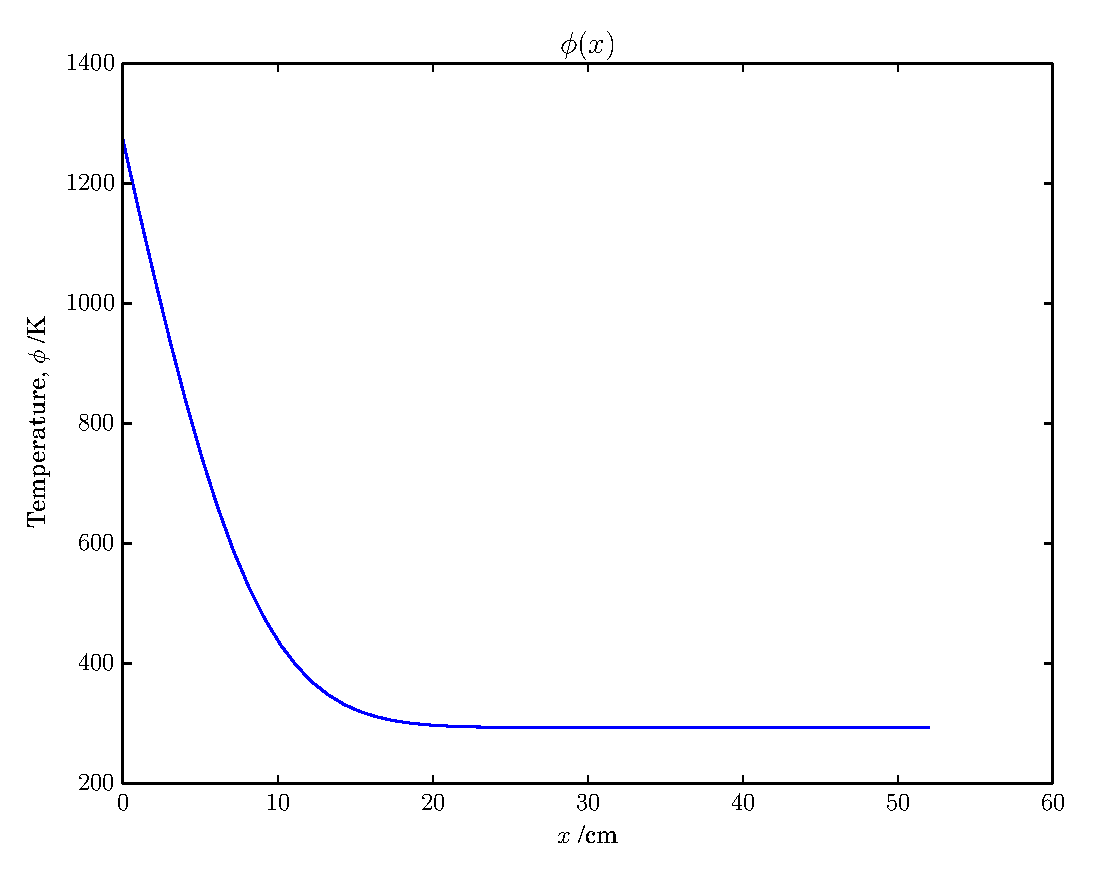
\includegraphics[width=0.5\linewidth]{graphs/diffusion/hot/t_100_rod_normal}
    }
    \caption{Temperature distribution along rod with one end in furnace at \SI{10}{\second} and \SI{100}{\second}.}
\end{figure}

\begin{figure}
    \ContinuedFloat
    \centering
    \subfloat[$t=$\SI{1000}{\second}]{
        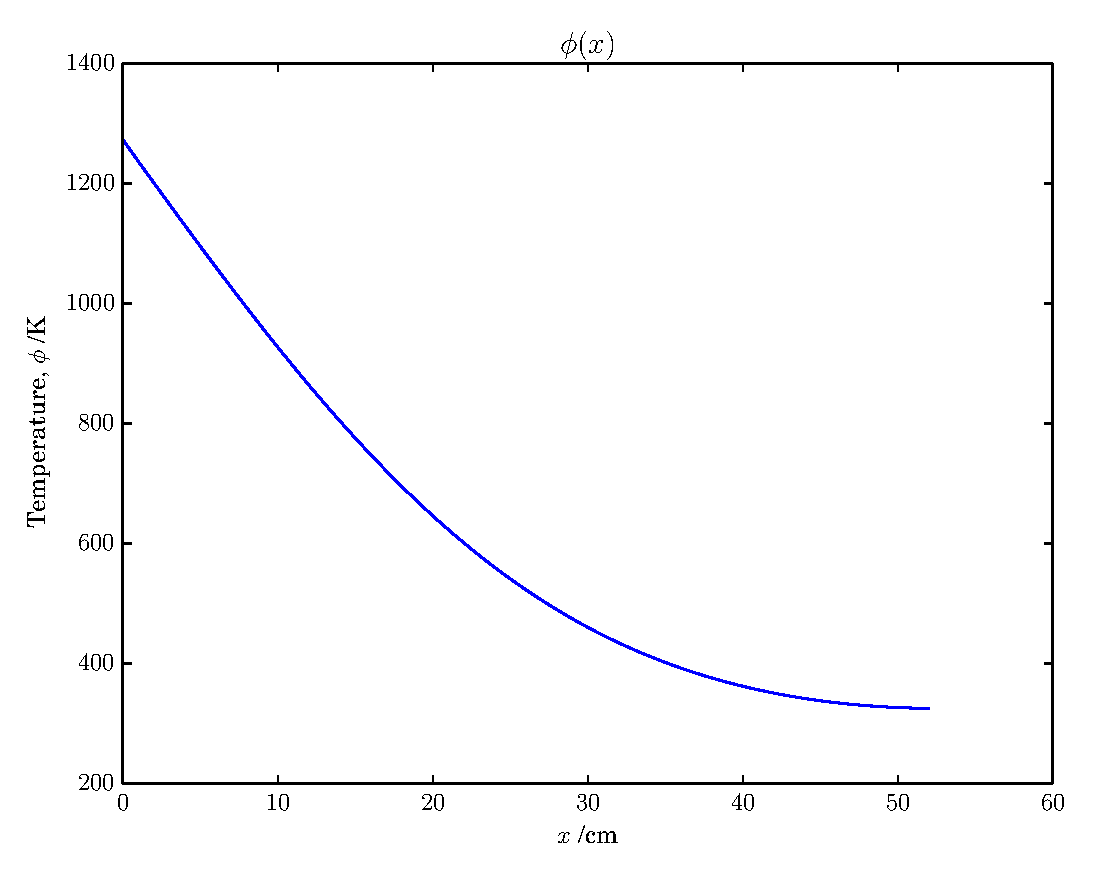
\includegraphics[width=0.5\linewidth]{graphs/diffusion/hot/t_1000_rod_normal}
    }
    \subfloat[$t=$\SI{10000}{\second}]{
        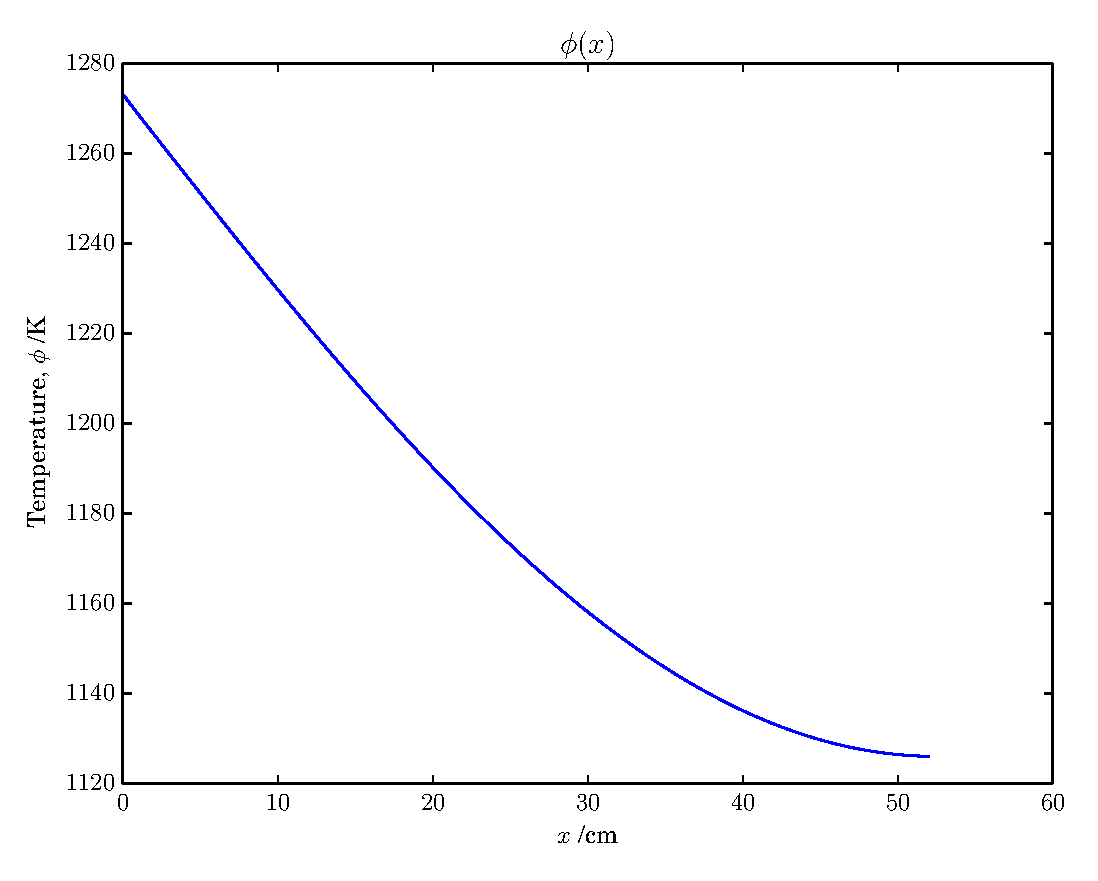
\includegraphics[width=0.5\linewidth]{graphs/diffusion/hot/t_10000_rod_normal}
    }
    \caption{Temperature distribution along rod with one end in furnace at \SI{1000}{\second} and \SI{10000}{\second}.}
    \label{fig:hot_diffusion}
\end{figure}

\subsection{Other end held in ice at \SI{0}{\celsius}}
\label{subsec:cold}

Once the other end of the rod is submerged in ice at \SI{0}{\celsius}, the time evolution of the temperature distribution of the rod drastically changes. Where before no true equilibrium can be found in finite time (ignoring floating point errors), the existence of the boundary condition of the ice means that after 7206.9 seconds, the system converges to an equilibrium state, where the temperature distribution function linearly falls off from \SI{1000}{\celsius} at one end to \SI{0}{\celsius} at the other end, as shown in Figure \ref{subfig:cold_t_10000}. The time advancement shown in Figure \ref{fig:cold_diffusion} is similar to that of \ref{fig:hot_diffusion}, however the fall-off is skewed at the right hand side due to the presence of the cold ice on the right end of the rod.

\begin{figure}
    \centering
    \subfloat[$t=$\SI{10}{\second}]{
        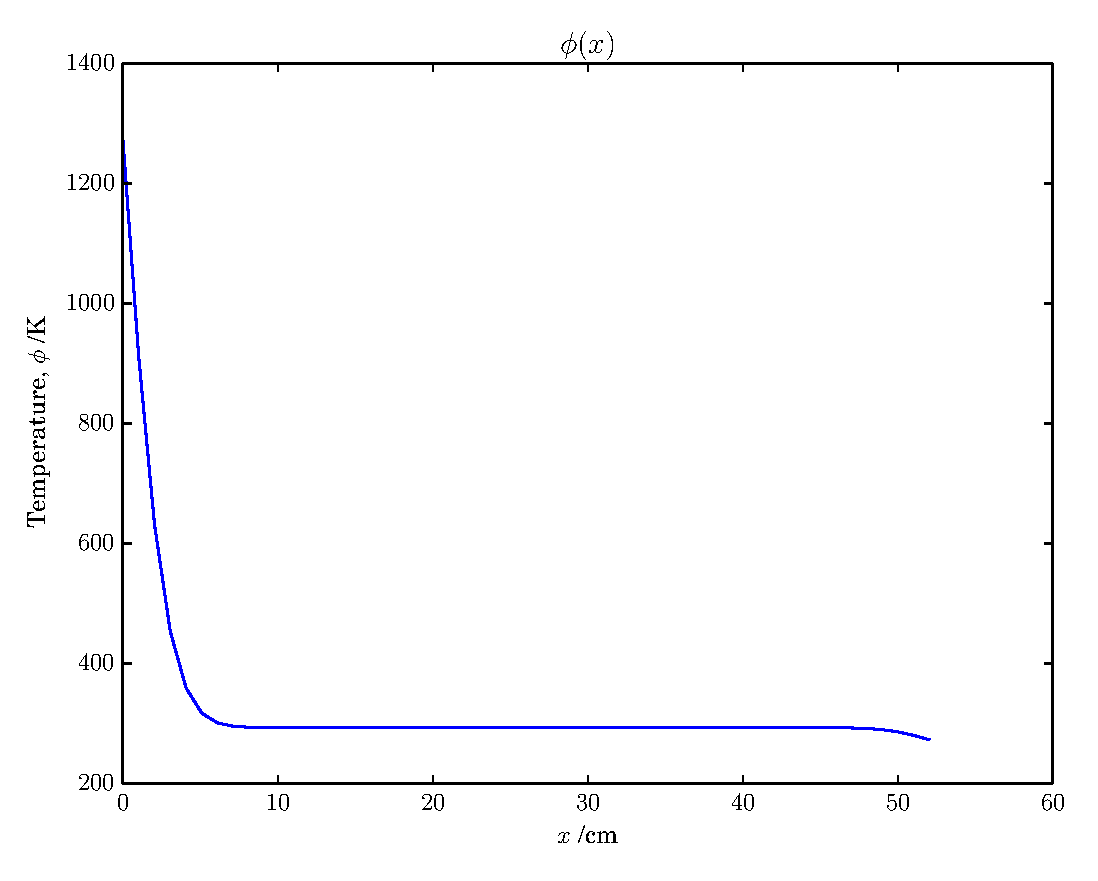
\includegraphics[width=0.5\linewidth]{graphs/diffusion/cold/t_10_rod_normal}
        \label{subfig:cold_t_10}
    }
    \subfloat[$t=$\SI{100}{\second}]{
        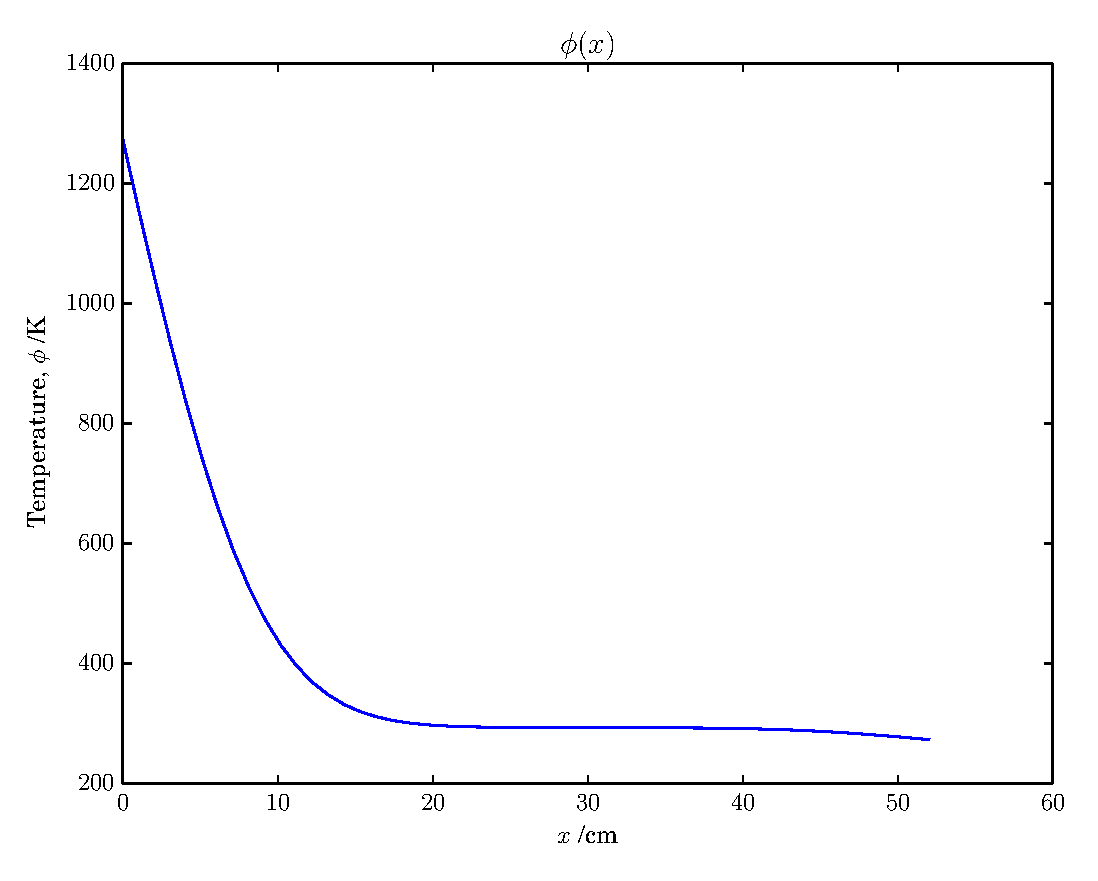
\includegraphics[width=0.5\linewidth]{graphs/diffusion/cold/t_100_rod_normal}
        \label{subfig:cold_t_100}
    }
    \caption{Temperature distribution along rod with one end in furnace and other in ice at \SI{10}{\second} and \SI{100}{\second}.}
\end{figure}

\begin{figure}
    \ContinuedFloat
    \centering
    \subfloat[$t=$\SI{1000}{\second}]{
        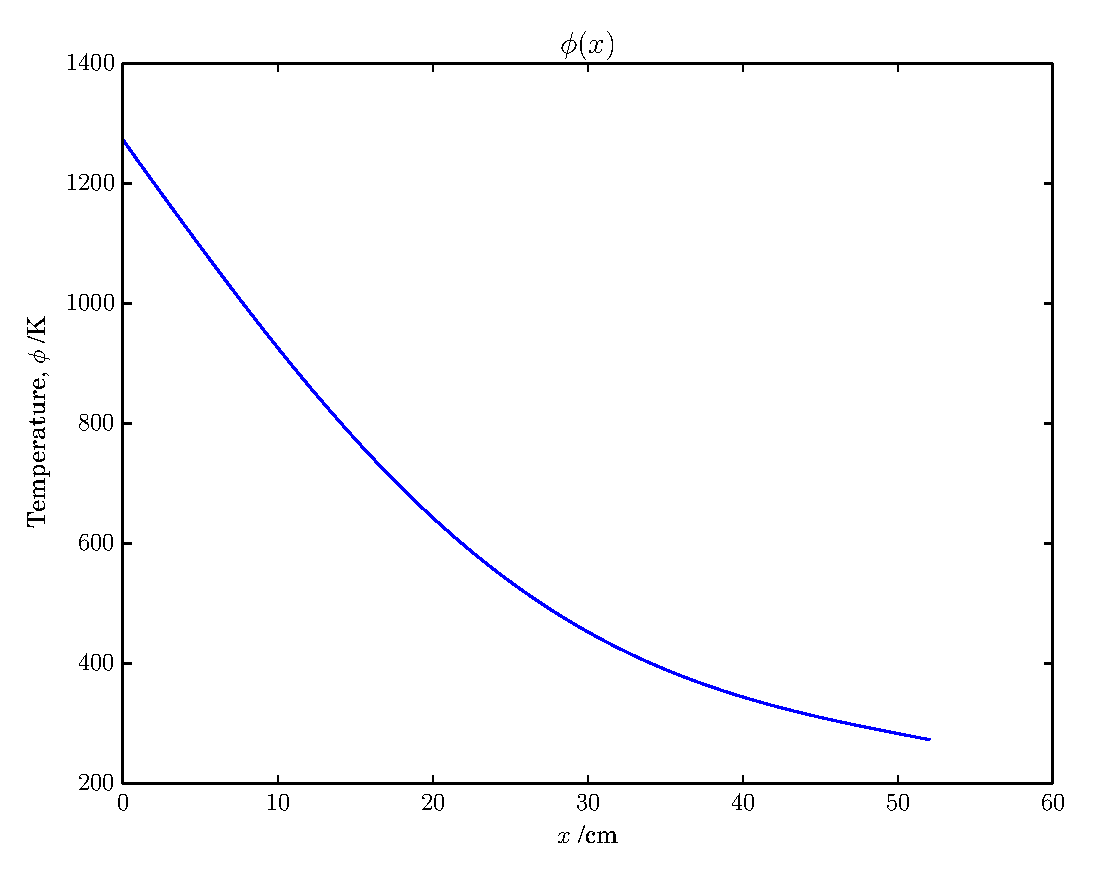
\includegraphics[width=0.5\linewidth]{graphs/diffusion/cold/t_1000_rod_normal}
        \label{subfig:cold_t_1000_normal}
    }
    \subfloat[$t=$\SI{10000}{\second}]{
        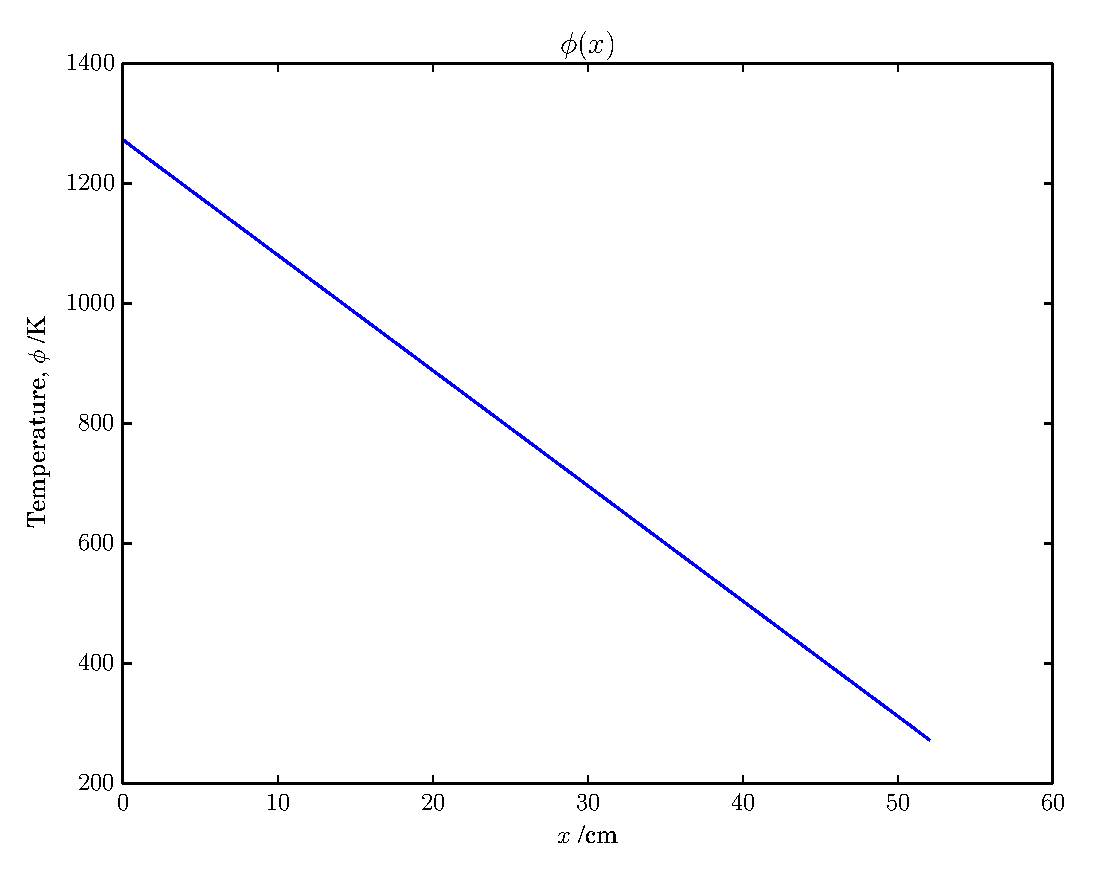
\includegraphics[width=0.5\linewidth]{graphs/diffusion/cold/t_10000_rod_normal}
        \label{subfig:cold_t_10000}
    }
    \caption{Temperature distribution along rod with one end in furnace and other in ice at \SI{1000}{\second} and \SI{10000}{\second}.}
    \label{fig:cold_diffusion}
\end{figure}

\subsection{Imposing Boundary Conditions}
\label{subsec:imposing_boundary_conditions}

Two boundary conditions need be imposed for this solution. The first type, Dirichlet boundary conditions, are the constant temperature regions, namely the $\phi(0,t)=\SI{1273.15}{\kelvin}$ for all $t$ in Section \ref{subsec:hot} and in addition $\phi(x_{\text{end}},t)=\SI{273.15}{\kelvin}$ for all $t$ in Section \ref{subsec:cold}. These are simple to impose as they can simply be set after every iteration. However, the second type of boundary conditions, the Neumann boundary conditions, are harder to implement. Here the Neumann boundary conditions are the no heat loss condition, which requires that $\frac{\partial \phi}{\partial x} = 0$ at the end of the rod. This is implemented by the altering of the top-left most and bottom-right most terms in the matrix of prefactors. Equation \ref{eqn:implicit}, giving the implicit BTCS method for iteration, gives a matrix of prefactors where every diagonal term is equal to $1+\frac{2\alpha\delta t}{h^2}$. The factor of 2 arises because the nearest two neighbours are taken into account. However, when talking about the first and last nodes, because no heat loss through the sides is desired, only the one neighbour should be taken into account and thus this term should be $1+\frac{\alpha\delta t}{h^2}$ instead. This takes the Neumann boundary conditions into account and removes the element of heat loss through the sides of the iron rod.

\subsection{Performance}
\label{subsec:performance}

In order to maximise the efficiency of the calculations, the matrix of prefactors is constructed and inverted in the main loop of the program. This means that this relatively processor intensive activity need take place only once at the beginning of the program, instead of whenever the system of linear equations is being solved to advance time by the time step at every iteration. This means instead of using \texttt{NumPy}'s \texttt{numpy.solve(a,b)} in every iteration, \texttt{numpy.linalg.inv()} is invoked once and in every iteration the rod at time $t$ is dotted with the inverse of the prefactor matrix to solve the set of linear equations and evolving time.

\section{Conclusion}
\label{sec:conclusion}

In conclusion, finite difference betweens are used to solve both Laplace's equation and the heat diffusion equation. The Laplace solution is then applied to the physical situation of a parallel plate capacitor, where it is shown that the infinite plate solution holds when the ratio of the width of the capacitor plates to the plate separation is sufficiently large. Finally the solution to the heat diffusion equation is applied to the case of an iron rod with one end in a hot furnace and the other end in and out of freezing water. It is demonstrated that only when one end is placed in ice that an equilibrium is found at finite time.

\begin{thebibliography}{99}

    \bibitem{edwards2004}
        Ron Edwards, Bruce H. Falvo and David C. Larson,
        \emph{Elementary Linear Algebra (5th edition)},
        Chapter 10: Numerical Methods,
        Page 578.
        Houghton Mifflin Company,
        2004.

    \bibitem{golub1996}
        Gene H. Golub and Charles F. Van Loan,
        \emph{Matrix Computations (3rd edition)}.
        Johns Hopkins University Press,
        1996.

    \bibitem{demmel1997}
        James W. Demmel
        \emph{Applied Numerical Linear Algebra},
        Chapter 6: Iterative Methods for Linear Systems,
        Page 290.
        Society for Pure and Applied Mathematics,
        1997.

\end{thebibliography}

\end{document}